\documentclass{article}

% Language setting
% Replace `english' with e.g. `spanish' to change the document language
\usepackage[english]{babel}


% Set page size and margins
% Replace `letterpaper' with `a4paper' for UK/EU standard size
% 
\usepackage[a4paper, left=1.4in, right=1.4in, top=1.2in, bottom=1.2in]{geometry}

% Useful packages
\usepackage{amsmath}
\usepackage{graphicx}
\usepackage[colorlinks=true, allcolors=blue]{hyperref}
\usepackage{apacite}
\usepackage[acronym]{glossaries}
\usepackage[nottoc]{tocbibind}
\usepackage{natbib}
\glstoctrue
\usepackage[⟨options⟩]{fancyhdr}
\usepackage{parskip}
\usepackage{adjustbox}
\usepackage{chngcntr}
\counterwithin{figure}{section}
\counterwithin{table}{section}



\title{Discovering City Perception by Mining Semantic Trajectory}
\author{Leyi Xu}

\makeglossaries
\newacronym{gcd}{GCD}{Greatest Common Divisor}
\newacronym{lcm}{LCM}{Least Common Multiple}
\newacronym{ugc}{UGC}{User-Generated Content}
\newacronym{nlp}{NLP}{Natural Language Processing}
\newacronym{msm}{MSM}{Multidimensional Similarity Measure}
\newacronym{muitas}{MUITAS}{Multiple-Aspect Trajectory Similarity Measure}
\newacronym{lda}{LDA}{Latent Dirichlet Allocation}
\newacronym{lsi}{LSI}{Latent Semantic Indexing}
\newacronym{plsi}{PLSI}{Probabilitistic Latent Semantic Indexing}
\newacronym{mallet}{MALLET}{MAchine Learning for LanguagE Toolkit}
\newacronym{tmt}{TMT}{Stanford Topic Modeling Toolbox}
\newacronym{poi}{POI}{Point of Interest}
\newacronym{api}{API}{Application Programming Interface}
\newacronym{aoi}{AOI}{Areas of Interest}
\newacronym{dbscan}{DBSCAN}{Density-Based Spatial Clustering of Applications with Noise}
\newacronym{tfidf}{TF-IDF}{Term Frequency-Inverse Document Frequency}

\begin{document}
\maketitle

% \chapter{Abstract}

\pagenumbering{roman}

\tableofcontents
\newpage

\listoffigures
\newpage

\listoftables
\newpage

\printglossary[type=\acronymtype]
\newpage

\pagenumbering{arabic}

\pagestyle{fancy}

 % ============================================ Introduction ============================================
\section{Introduction}
\subsection{Motivation}
How are cities distinguished from each other? The physical properties, like landmarks, road networks, and city structures, make the city distinctive. For instance, speaking of London, it is easy for people to come up with the London Eye, the Tower of London, Big Ben, etc. The city, however, is not only constituted by its physical properties, it is also a large human settlement \citep{goodall_penguin_1987,kuper_social_2013}. In his book “The Image of the City”, Kevin Lynch proposed the concept of the imageability of the city and discussed how the mental image is related to the physical qualities of the city \citep{lynch_image_1960}. According to the city perception survey  \underline{(Institute for Urban Strategies, 2020)}, the most frequent words used to describe London are Expensive, History, Big Ben, Culture, and Rain. People tend to describe the city based on what they see and experience, and how they feel about it rather than merely listing famous attractions. To better understand the city, it is far from enough to know only its physical properties. People interact with these physical properties and it is their mental images generated during the interaction that makes the city distinguished from others. Building the city perception map can enhance the city's characteristics, and helps to discover its uniqueness.

Social media data has become an increasingly popular source for discovering the city, as users can post spatially and temporally referenced information on platforms such as Twitter \footnote{\url{https://twitter.com/home}}, Flickr \footnote{\url{https://www.flickr.com/}}, and Foursquare \footnote{\url{https://foursquare.com/}}. The large number of Foursquare check-ins generated by users, for example, can be used to investigate how people move around the city \citep{ferreira_beyond_2015}, providing valuable insights into urban mobility patterns. Additionally, \acrfull{ugc} on social media platforms, like images, reviews, and \acrfull{poi}, offers the potential to extract city perception in a bottom-up approach, as people share their experiences and observations of different cities. Therefore, social media data can provide a precise and rich source of information for discovering and understanding cities.

The city perception is not static, it varies both spatially and temporally, which can even differ among different population groups. To reflect the dynamic nature of city perception, one can investigate people's movements. Spatially and temporally referenced social media data can enhance the study on human mobility \citep{beiro_predicting_2016}, particularly in constructing trajectories that provide semantic information about people's visiting purposes and impressions of the city. This extracted city perception is more akin to a city image that reflects the distinctiveness of the city, making it more attractive to people and resources. In an urban context, this perception can supplement public surveys to understand citizens’ needs and preferences. The abundance of social media data makes it possible to divide users into different population groups, and their city perceptions help to create a more livable city for people of diverse ages and socio-economic backgrounds. Thus, social media data offers a powerful tool for improving the quality of life for urban residents.

\subsection{Research Questions}
The city perception is typically collected through surveys involving a large number of participants, which can be labor-intensive and time-consuming. With the emergence of social media data, many studies have turned to \acrshort{ugc} to gain insight into how users perceive a city \citep{cranshaw_livehoods_2021,huang_user_2022}. However, while most studies put focus on specific regions of the city, little research has been conducted on city perception based on trajectories. Identifying meaningful places is a prerequisite for constructing trajectories. A place should not be merely a random point, but rather a space where people interact, with attributes based on human consensus. For instance, an area with grass and trees may not necessarily be considered a place, but if it attracts people and offers functionality for leisure purposes, it becomes a place. Using social media data, places can be identified based on users’ frequently visited locations. The Foursquare check-ins are often used to identify popular landmarks in a city \citep{ferreira_beyond_2015,ferreira_uncovering_2020,santos_uncovering_2018}. Foursquare venue names and categories enrich check-ins with attributes, making them more like places. In addition to these objective attributes, subjective attributes are also worth exploring. Flickr allows users to add tags to their photos, which can be a valuable source of data to enrich place attributes.

The trajectory is the chronological representation of people’s movements. Efforts have been made to extract movement patterns from trajectories to reveal the underlying visiting preferences \citep{vu_discovering_2019}. However, the trajectory should not be limited to geometric movements, the semantic information underlying trajectories is also valuable for exploration. When the semantic information of a trajectory is combined with its spatial and temporal data, it is referred to as a semantic trajectory \citep{yan_semantic_2011}. To understand visitor behaviors, most studies on semantic trajectories annotate the trajectories with attributes such as time, weekday, weather, etc. \citep{cai_mining_2018,petry_towards_2019}. However, in existing studies, the enrichment of semantic information for trajectories through place attributes has not been adequately considered. Semantic trajectories can vary across different groups of people, with locals and tourists organizing their trips differently based on local knowledge and online travel reviews. Moreover, different time spans can also result in different semantic trajectories, as people tend to have different visiting behaviors on weekdays and weekends. While existing studies have primarily focused on the visiting behaviors of locals and tourists \citep{domenech_using_2020,straumann_towards_2014}, the city perception of locals and tourists in different scenarios, like different time spans, is still under investigation.

To bridge the gap, this study aims to construct the semantic trajectories of locals and tourists in Greater London with Foursquare check-ins and Flickr tags. Greater London is an English-speaking city that attracts numerous tourists every year. Moreover, there are lots of Foursquare and Flickr users sharing check-ins and photos in Greater London, which lays the foundation for semantic trajectory construction. This study examines two research questions:

\textbf{RQ1: What’s the functionality of the place based on the visit number of locals and tourists?}

Given the varying functionalities of different places, they tend to attract diverse populations with specific visiting objectives. To investigate the distribution of places that cater to distinct population groups, it is imperative to assess the degree of mixture between locals and tourists in these places \citep{li_analyzing_2018}. This evaluation can identify places that appeal to both locals and tourists, as well as those that primarily attract one group or the other. By combining this evaluation with the semantic attributes of places, the visiting objectives of locals and tourists can also be revealed for different place types.

\textbf{RQ2: How do locals and tourists perceive the city along their semantic trajectories at different time spans?}

The perception of a city is subjective and can vary among both locals and tourists, with changes over time. To investigate city perception more accurately, constructing semantic trajectories that consider both population groups and time spans is useful. Specifically, semantic trajectories of locals and tourists during different times of day and week, including daytime and nighttime, as well as weekdays and weekends, will be constructed. By incorporating the semantic attributes of places into these trajectories, the city perception of both locals and tourists at various time spans can be interpreted and compared.
\newpage

% ============================================ ||| Related Work||| ============================================
\section{Related Work}
% ============================= || City Perception || =============================
\subsection{City Perception}
% ====================== | UGC in City Perception | ======================
\subsubsection{UGC in City Perception}
% ============== specific perception ==============
City perception, which refers to how people experience and interact with the urban environment, has significant implications for the city's vitality and is a critical topic in the field of urban planning and design \citep{jacobs_death_1961}. The large volume of \acrshort{ugc} available online makes data collection cost-effective, and it has proven to be a valuable data source for gaining insights into public perceptions of cities. City perception research encompasses studies that aim to improve specific subjects within the city, as well as those that focus on understanding general city perception. Among studies that focus on specific subjects, landscape amenities have received widespread attention. For example, \cite{huang_user_2022} utilized Google Maps reviews to evaluate park performance and user experience, which showed the potential of using these reviews to enhance urban landscapes. There are also some studies investigating the soundscape of parks, as city perception can be reflected from an acoustic perspective. Such studies mainly focus on the evaluation of acoustic comfort and people's acceptability of the urban environment \citep{tse_perception_2012, liu_effects_2014}. Urban safety is another popular topic in city perception research. Some cities, despite being popular tourist destinations, suffer from natural disasters or negative publicity about crime, making perceived danger a worthy topic of investigation. \cite{yao_towards_2020} applied Tweets to build a real-time urban analytical and geo-visual system to provide early alerts for crises and emergencies. \cite{yang_crimetelescope_2018} collected crime data and Tweets to predict and visualize crime hotspots.

% ============== tourist interest - grid and AOI scale ==============
In studies aimed to investigate general city perceptions, analyses are carried out to identify popular areas at various spatial scales. A grid-based approach has been employed to detect tourist attractions. The study area is divided into equal-sized grids, and the concentration of \acrshort{ugc} within grids is measured. Spatial autocorrelation indices, such as Moran's I and Getis-Ord G statistics, were usually used to identify spatial clusters of tourism activities \citep{garcia-palomares_identification_2015, kim_coastal_2021}. Some studies go beyond exploring the distribution of tourist hotspots and extract semantic information from these hotspots. For example, \cite{li_analyzing_2018} created the location-based word-cloud maps with Flickr tags to better identify the exact attractions in each cluster, enriching aspects of city perception. \cite{bahrehdar_description_2018} delved deeper into Flickr tags by generating semantic topics with topic modeling, and labeled grids with meaningful topics to map users' perception of the space. A non-grid-based approach can also be utilized to discover the spatial patterns of tourist attractions. For instance, Tweets, Flickr images, and Foursquare check-ins were used to detect \acrfull{aoi} with clustering techniques such as K-Means clustering, \acrfull{dbscan}, and self-developed algorithms \citep{hu_extracting_2015, hasnat_identifying_2018, cranshaw_livehoods_2021}. There are also studies extracting semantic information associated with \acrshort{aoi}. \cite{dunkel_visualizing_2015} clustered Flickr images and subsequently mapped the tags associated with each cluster, with the size reflecting the frequency, which presented a comprehensive overview of people's perceptions of the study areas. \cite{zhou_detecting_2015} applied \acrshort{dbscan} to detect Flickr images communities and then employed random forest to classify Flickr tags into three categories based on the spatial, temporal, and user features. This helped describe detected communities with more precise word clouds. \cite{jailani_machine_2021} used \acrfull{tfidf} to assign weights to keywords of Flickr data, including tags, titles, and descriptions, and utilized \acrshort{dbscan} to cluster weighted keywords, thus the discovered \acrshort{aoi} were integrated with intrinsic semantic information. \cite{santos_uncovering_2018} collected reviews about places from Google Places and Foursquare tips, and generated perception maps to uncover how the urban outdoor areas were expressed in social media.

% ============== tourist interest - trajectory scale ==============
Constructing trajectories serves as an alternative approach to discovering how visitors perceive a city, as it reflects their movement patterns. \cite{girardin_digital_2008} utilized people's mobile phone calls and Flickr images to investigate the visitor flows among major visitor attractions in Rome, Italy. They applied the Origin-Destination matrix to understand the preferences of visitors. Some studies use the trajectory network to detect the movement patterns of visitors. The weighted network graph was constructed from the clusters of Flickr and Twitter data, and then the network analysis like betweenness and eigenvector centrality was performed to extract popular attractions and routes \citep{straumann_towards_2014, hu_graph-based_2019}. Some studies construct trajectories based on the street layout. For example, \cite{mohino_identifying_2018} identified the main tourist routes of Flickr users along the street network, and \cite{domenech_using_2020} established the hierarchy of the street network based on the number of trajectories passing through. This helped to better understand the city structure and context. \cite{yin_diversified_2011} also ranked the street-based trajectories with various ranking methods, which contributed to the location recommendation at the trajectory level. Researchers have attempted to construct semantic trajectories to interpret the movement patterns more meaningfully. Different from raw trajectories that only contain spatial and temporal information, semantic trajectories are also annotated with higher-level semantic information at each point. \cite{wan_semantic-geographic_2017} took the venue categories of Sina check-ins into consideration when building users' semantic-graphic traces, and detected their movement patterns with a density-based clustering algorithm. In order to gather further insights into visitors' characteristics and activity preferences, topic modeling was used to analyze the venue categories of their check-ins \citep{vu_discovering_2019, ferreira_uncovering_2020}. In addition to the venue category, the weather and time were also considered in the construction of semantic trajectories \cite{cai_mining_2018, liu_stccd_2020}.


% ====================== | Topic Modeling of UGC | ======================
\subsubsection{Topic Modeling of UGC}
\acrfull{nlp} has emerged as a powerful tool for information retrieval. Within \acrshort{nlp}, topic modeling has become increasingly popular in recent years, especially in text mining for \acrshort{ugc}. Topic modeling branches off from the area of generative probabilistic modeling and is used to identify latent themes within a large corpus. Given a set of documents,  topic modeling allows researchers to gain insights into topics being discussed by people \citep{sui_inferring_2013}. In topic modeling, a \textit{word} or \textit{term} is a single token, which is the fundamental unit of individual data. A \textit{document} refers to a piece of text comprising multiple words. A \textit{corpus} is a collection of documents and serves as the basis for topic modeling. A \textit{vocabulary} represents all distinct words in a corpus. A \textit{topic} is a latent theme discovered in topic modeling, and it is characterized as a probability distribution spanning a given vocabulary \citep{vayansky_review_2020}. Figure~\ref{fig:topic_modeling} shows the process of topic modeling. With the corpus as the input, topic modeling is performed to generate a set of topics, each of which represents a cluster of words with the probability of belonging to the topic. Furthermore, the results of topic modeling include the distribution of topics in each document, which indicates the degree of association between the topics and the document, as well as the frequency of words within each topic. The origin of the topic model is \acrfull{lsi} proposed by \cite{papadimitriou_latent_2000}, but \acrshort{lsi} is not a probabilistic model. To address this limitation, \cite{hofmann_unsupervised_2001} introduced \acrfull{plsi} and subsequently, \cite{blei_latent_2003} proposed \acrfull{lda}, which is a more complete generative probabilistic model \citep{liu_overview_2016}. Compared with \acrshort{plsi}, \acrshort{lda} generates better disambiguation of words and more precise identification of topics in documents due to its consideration of a sparse Dirichlet prior in the topic distribution \citep{barde_overview_2017}.

The \acrshort{lda} method has demonstrated its usefulness as a valuable tool for understanding unstructured data. \acrshort{lda} assumes that a document contains a randomized combination of latent topics. To generate the document, a K-vector \(\theta\) that represents the mixture proportion of \(k\) topics is sampled3 with a Dirichlet prior distribution \(p(\theta|\alpha)\). The variable \(k\) specifies the dimension of the distribution and also the dimension of the topic variable \(z\), which defines the total number of topics generated by the model. A Dirichlet variable \(\theta\) with a dimension of \(k\) can take values in the \((k-1)\)-simplex and has a probability density on this simplex, which is determined by the following equation:

\begin{equation} \label{eq:lda}
    p(\theta|\alpha)\ = \frac{\Gamma(\sum_{i=1}^{k} \alpha_{i})}{\prod_{i=1}^{k}\Gamma(\alpha_{i})}\theta_{1}^{z_{1}-1}...\theta_{k}^{z_{k}-1}
\end{equation}

In Equation \ref{eq:lda}, the parameter \(\alpha\) is the hyperparameter of the Dirichlet distribution, representing a prior count of the frequency of an individual topic appearing in a document. Figure~\ref{fig:lda} illustrates the generative process of \acrshort{lda}. The parameter \(\beta\) is also a Dirichlet prior hyperparameter that determines the degree of smoothing over word distributions in all topics. The values of \(\alpha\) and \(\beta\) are chosen based on the size of the vocabulary and the number of topics selected \citep{blei_latent_2003}. Optimizing these parameters is crucial to obtain meaningful results from this method \citep{vayansky_review_2020}. In practice, several tools are available for implementing the \acrshort{lda} model. \acrfull{mallet} \footnote{\url{https://mimno.github.io/Mallet/index}} is a Java-based package that provides efficient and sampling-based implementations of \acrshort{lda} related models. Gensim \footnote{\url{https://pypi.org/project/gensim/}} is a Python library that implements popular topic modeling algorithms, including \acrshort{lda} and \acrshort{lsi}. \acrfull{tmt} \footnote{\url{https://downloads.cs.stanford.edu/nlp/software/tmt/tmt-0.4/}} is another tool that trains topic models to create summaries of the text. An evaluation of \acrshort{mallet} and Gensim was conducted to compare their performances \citep{ebeid_mallet_2016}. To facilitate the interpretation of \acrshort{lda} results, \cite{sievert_ldavis_2014} developed LDAvis \footnote{\url{https://github.com/cpsievert/LDAvis}}, a web-based interactive visualization of topics. LDAvis allows users to select a topic to reveal the most relevant terms for that topic. Users can also select a term to reveal its conditional distribution over topics (Figure~\ref{fig:ldavis}). LDAvis leverages the R language, specifically the shiny package, to enable users to visualize topics. Additionally, a Python library, pyLDAvis \footnote{\url{https://github.com/bmabey/pyLDAvis}} was developed to provide interactive topic model visualization in Python, which is a port of the R LDAvis package.

Topic modeling using \acrshort{lda} has been widely adopted for extracting information from \acrshort{ugc}. For instance, Flickr tags have been utilized for investigating the properties of places and semantic similarity of streets \citep{bahrehdar_description_2018, bahrehdar_streets_2020}. In addition, the venue categories of Foursquare check-ins have been used to extract semantic information about places. The \acrshort{lda} has been employed to the venue categories of users' check-ins along their movements to depict different types of users with distinct character profiles \citep{ferreira_uncovering_2020} and discover implicit activity preferences of users \citep{vu_discovering_2019}. Furthermore, Google reviews have been found to be a good data source to extract leisure activity potentials in urban space \citep{van_weerdenburg_where_2019}.


\begin{figure}
\centering
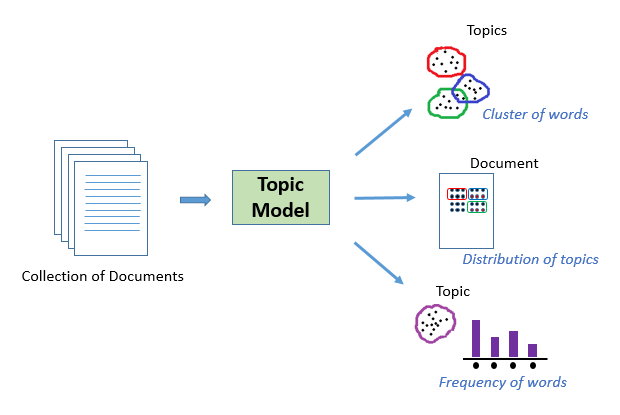
\includegraphics[width=0.7\textwidth]{figures/topic_modeling.png}
\caption{\label{fig:topic_modeling}Framework of topic modeling \citep{usmani_natural_2021}.}
\end{figure}

\begin{figure}
\centering
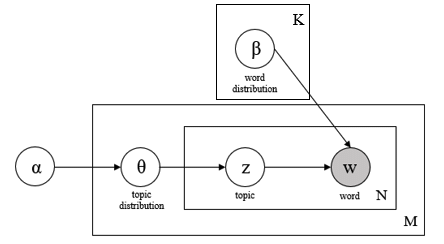
\includegraphics[width=0.7\textwidth]{figures/lda.png}
\caption{\label{fig:lda}Illustration of the LDA generative process. The outer box M denotes the repeated sampling for each document and the inner box N represents sampling within each document. The box K represents sampling for each topic \citep{vayansky_review_2020}.}
\end{figure}

\begin{figure}
\centering
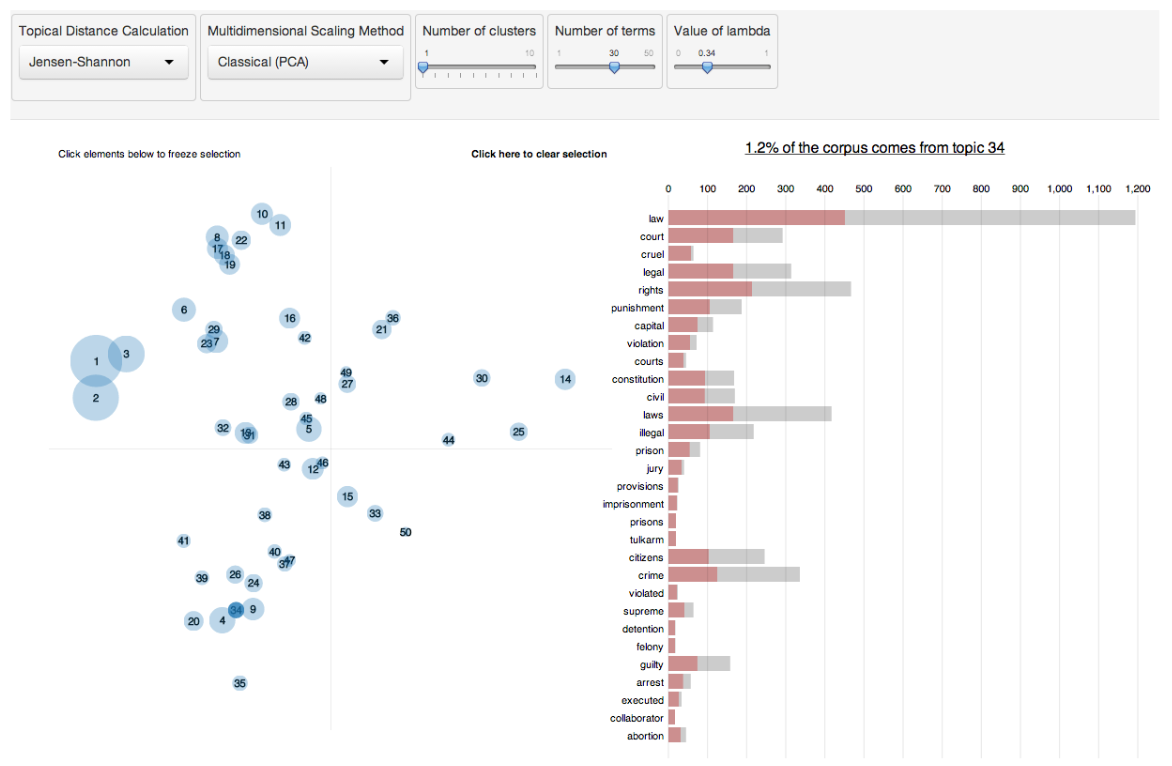
\includegraphics[width=1\textwidth]{figures/ldavis.png}
\caption{\label{fig:ldavis}The layout of LDAvis \citep{sievert_ldavis_2014}.}
\end{figure}

% ====================== | Identification of Locals and Tourists | ======================
\subsubsection{Identification of Locals and Tourists}
Distinguishing between locals and tourists is crucial when investigating how different people perceive a city. Locals and tourists might have various preferences and behaviors while visiting a city, and analyzing their patterns separately can yield valuable insights. The time interval is a commonly used indicator for identifying locals and tourists. Typically, locals are assumed to stay in the city for longer periods than tourists. Researchers have used the time interval between a user's first and last posts within a city boundary on social media platforms to estimate the length of his stay, with time intervals ranging from 10 days to 30 days \citep{girardin_digital_2008, hu_graph-based_2019, hopken_flickr_2020}. For example, given a 30-day threshold, a Twitter user whose first and last Tweets were posted within a 20-day time interval would be classified as a tourist. However, it is important to note that some locals may share content only for short periods, and some tourists may stay longer and continue sharing content. Another indicator of determining locals and tourists is user profiles. Social media platforms like Foursquare, Flickr, and Twitter, offer \acrshort{api} to collect user profiles containing information on their city of residence and hometown. Previous studies have demonstrated the feasibility of using these profiles to identify users' origins \citep{ferreira_beyond_2015, li_analyzing_2018}. However, this approach has some limitations, as many users may leave their profiles incomplete without providing the city of residence. \cite{ferreira_uncovering_2020} combined both the time interval and user profiles to overcome these limitations. If a user's time interval suggests that he is a local, but his profile indicates that he is from another city, he would be classified as a tourist. There are also other indicators for the identification of locals and tourists. In addition to the time interval, \cite{hallot_who_2015} also analyzed the categories of the place visited and the frequency of visits within the same place to extract tourists. \cite{yang_identifying_2021} assumed that locals and tourists might have different numbers of Foursquare check-ins, total travel distances, and time intervals, and applied K-means clustering to separate users into locals and tourists based on the above indicators. \cite{hasnat_identifying_2018} used the number of Tweets within the geographical boundary as an indicator to identify tourists. For example, if a user posted fewer Tweets within the geographical boundary of Florida between 12 am and 6 am than outside the boundary, he would be assumed as a local. Overall, these approaches help researchers to effectively differentiate between locals and tourists, enabling them to investigate the visiting behaviors of different groups of people.


% ============================= || Place || =============================
\subsection{Place}
% ====================== | Place Conceptualization | ======================
\subsubsection{Place Conceptualization}
City perception can be shaped by individuals' perceptions of various places. To explore place-based perception, the first step is to conceptualize the place. According to \cite{tuan_place_1975}, place is created by human beings for human purposes, and it encompasses not only geometrical and ideographic perspectives but also an experiential perspective. It is important to distinguish between space and place. Space is defined as a continuous and unrestricted area that can be free to use or occupied, moreover, it is abstract and lacks content. While place is a segment of geographical space loaded with human meaning, offering the potential for human interaction \citep{tuan_place_1975, agnew_space_2011, cresswell_place_2014}. \cite{relph_place_1976} developed an \textit{insideness} scale to illustrate the social relationships of a place, which includes the knowledge of the physical details of place, sense of connection with a community, and a personal connection with place. Moreover, \cite{williams_measurement_2003} employed the place attachment \citep{altman_place_1992} as the scale to identify and measure the meanings of places based on the place identity \citep{proshansky_city_1978,proshansky_place_1983} and place dependence \citep{stokols_people_1981}. As the definition of place has evolved, researchers have contributed to the conceptualization of place dimensions. \cite{jorgensen_comparative_2006} described place with three dimensions: (1) place-specific beliefs, also known as place identity, (2) emotions, or place attachment, and (3) behavioral commitments or place dependence. \cite{agnew_space_2011} conceptualized the place with three dimensions: (1) location, which refers to the physical position of a place represented by its toponym and coordinates, (2) locale, which encompasses the properties and affordance of a place, and (3) sense of place, which is associated with the sentiments and emotions of individuals who visit the place \citep{bahrehdar_description_2018}. It is noteworthy that according to the affordance theory, affordance can shape behavior and guide actions of individuals \citep{gibson_theory_1977}, thus the affordance of place can influence how people perceive it. \cite{wartmann_characterizing_2016,wartmann_describing_2018} refined the aspect of the locale with categories of landscape elements.

% ====================== | Place Categories/Locale | ======================

tourist-functional relations of urban places, venue categories, network graph - Foursquare: \cite{yang_identifying_2021}

Furthermore, places are categorized to discover the relationship between different categories of places. \underline{\cite{liu_stccd_2020}} constructed the location category hierarchy tree based on daily purposes, where the main categories include (1) work/study, (2) food, (3) entertainment, (4) traffic, and (5) live. \cite{koirala_social_2015} categorized places based on tourism ontologies, which include (1) leisure, (2) restaurant, (3) attraction, (4) emergency service, (5) transport, (6) accommodation, and (7) other buildings. Foursquare also provides 10 venue categories, and an increasing number of studies adopt and recategorize the Foursquare venue categories to represent places \cite{ferreira_uncovering_2020,yang_identifying_2021}.

% ====================== | Sense of Place | ======================
Surveys cab be used to collect people's emotional relationships with places to understand their positive or negative experiences \citep{manzo_for_2005}. \acrshort{ugc} also demonstrates the potential for exploring places. \cite{wang_using_2015} used Foursquare check-ins to evaluate the performance of four different clustering algorithms in identifying meaningful places. \cite{sui_inferring_2013} applied \acrshort{lda} to georeferenced travel blogs to generate meaningful topics describing places. \cite{hallot_who_2015} combined Google Place reviews and Foursquare check-ins to retrieve place-based semantics, enabling the inference of additional information about users based on their movements.

 
% ====================== | Place Popularity Measurement| ======================
\subsubsection{Place Popularity Measurement}
a generalized index of dissimilarity \cite{sakoda_generalized_1981}

difference ratio \cite{li_analyzing_2018}

top-ranked locations, location importance: \cite{yin_diversified_2011}

venue categories - Foursquare: \cite{ferreira_uncovering_2020}

semantic trajectory clustering, trajectory similarity, community detection >>> clustering, network graph - Flickr + Foursquare: \cite{liu_stccd_2020}

place categories, table 1 - Flickr: \cite{donaire_tourist_2014}


% ============================= || Trajectory || =============================
\subsection{Trajectory}

% ====================== | Urban Mobility | ======================
\subsubsection{Urban Mobility??}
tourist movement patterns, network graph, Markov clustering: \cite{hu_graph-based_2019}

tourists' behavior, network graph, ranking of places, locals and tourists comparison - Foursquare: \cite{ferreira_beyond_2015}

reconstruct narratives from georeferenced photographs, place and narrative, network analysis, community detection - Flickr: \cite{straumann_towards_2014}

digital footprint, mobile phone data + tickets sold + Flicker photos: \cite{girardin_digital_2008}

activity preferences, trajectory, topic modeling (venue types) - Foursquare: \cite{vu_discovering_2019}

tourists' movement patterns, clustering, GSP algorithm - Flickr: \cite{hopken_flickr_2020}

semantic trajectory, urban mobility patterns, OD matrix - Foursquare: \cite{nin_tweets_2014}

identifying tourist main routes, focus on real trajectory patterns along the street network - Flickr: \cite{mohino_identifying_2018}

tourist-functional relations of urban places, venue categories, network graph - Foursquare: \cite{yang_identifying_2021}

\underline{important!!!: \cite{parent_semantic_2013}}

% ====================== | Semantic Trajectory Construction | ======================
\subsubsection{Semantic Trajectory Construction}
definition of semantic trajectory

\underline{add the figure to show semantic trajectories}

refer to the definition of semantic trajectories in this literature: \cite{yan_semantic_2011}, \cite{parent_semantic_2013}

semantic trajectory pattern mining, similarity measure - Sina Weibo: \cite{wan_semantic-geographic_2017}

network analysis - Foursquare: \cite{ferreira_uncovering_2020}

visitor trajectories in world heritage cities, street - Flickr: \cite{domenech_using_2020}

Constructing spatial and temporal trajectories of different groups of people, like locals and tourists or visitors with different nationalities, has been a widely used approach to investigating visiting behaviors of people in the city \cite{straumann_towards_2014, ferreira_beyond_2015}. Attempts have been made to study trajectories by taking semantic descriptions into consideration. \cite{girardin_digital_2008} used Flickr data to extract the movement patterns perceptions of locals and tourists in Roma. \underline{\cite{vu_discovering_2019}} tried to find the hidden activity preferences in travel trajectories by applying topic modeling to Foursquare categories. Some studies go one step further by constructing semantic trajectories. The majority of these studies assign attributes, such as place type, day of the week, time, and weather, to place points in trajectories to represent the semantic information \cite{petry_towards_2019,liu_stccd_2020}. \underline{\cite{vu_discovering_2019}} summarized techniques for trajectory construction as the origin-destination matrix, network graph visualization, Markov chain, sequential pattern mining, and social network analysis. Among these techniques, the sequential patterns reveal typical trajectories where people largely visited. To mine sequences, the trajectory similarity should be  measured, and the Longest Common Sequence (LCSS) \cite{vlachos_discovering_2002}, and Edit Distance on Real sequence (EDR) \cite{chen_similarity_2005} are commonly used similarity measures. Given the similarity, trajectories can be clustered to extract typical ones with densely-based, hierarchical-based, spectral-based, and community-based trajectory clustering methods \cite{liu_stccd_2020}.


% ====================== | Sequential Pattern Mining | ======================
\subsubsection{Sequential Pattern Mining}

spatiotemporal trajectories:
Trajectory comparison - trajectory similarity measures \cite{tao_comparative_2021}: LSED, DTW, EDR, LCSS, DFD, FD

semantic trajectory pattern mining, similarity measure - Sina Weibo: \cite{wan_semantic-geographic_2017}

trajectory pattern ranking, prefixSpan algorithm - Flickr:  \cite{yin_diversified_2011}

tourists' movement patterns, clustering, GSP algorithm - Flickr: \cite{hopken_flickr_2020}

\underline{refer to Sequential Pattern Mining: A Survey in zotero}

spatiotemporal semantic trajectories

drawbacks of commonly used similarity measures, and the advantages of the similarity measure used in this study, refer to table 1 in \cite{petry_towards_2019} - Foursquare

semantic trajectory clustering, trajectory similarity, community detection >>> clustering, network graph - Flickr + Foursquare: \cite{liu_stccd_2020}

similarity measure option 1:
\cite{petry_towards_2019}

similarity measure option 2:
\cite{ferrero_mastermovelets_2020}

similarity measure option 3:
\cite{furtado_multidimensional_2016}, multidimensional similarity measuring

Other references:
\cite{xiao_inferring_2014}

Cite it!
@misc{petry2019trajminer,
  title={Trajminer},
  author={Petry, Lucas May and others},
  year={2019},
  howpublished={\url{https://trajminer.github.io}},
}


% ============================= || Research Gaps || =============================
\subsection{Research Gaps}
The previous studies illustrate the possibility of constructing semantic trajectories with social media data. Though both the texts and images have been applied to discover the city perception, there is limited research that integrates the place attributes into semantic trajectory construction. In the context of urban planning, the improvements of the regions should refer to people’s perception of important nodes, which are places in our case. While existing approaches of semantic trajectories construction are not entirely suited for exploring the perception from the place-based perspective. This study leverages social media data to capture the semantic information in people’s movement patterns by considering the place dimensions in trajectory construction.
\newpage
% ======================================================================================================


% ============================================ ||| Study Area and Data Preprocessing||| ============================================
\section{Study Area and Data Preprocessing}
\subsection{Study Area}
The study area is located in Greater London. As an English-speaking
city, Greater London covers an area of 1,572 \(km^2\) and has a population of 9.5 million inhabitants. According to tourism statistics of City of London, before the Covid-19 pandemic, Greater London attracted approximately 21 million visitors annually from across the world. Of these, 19.7 million visitors were day trippers, while 1.3 million visitors stayed overnight. The high volume of visitors makes Greater London an ideal location for studying the city perception of both locals and tourists. The boundary of Greater London used in this study was obtained from \href{https://data.london.gov.uk/dataset/statistical-gis-boundary-files-london}{LONDON DATASTORE} website.

\subsection{Data Preprocssing} 
Foursquare data and Flickr data in Greater London from April 3, 2012 to September 16, 2013 were collected with Python 3.9.12 to investigate how people move around the city and how they perceive it.

To investigate the city perception of locals and tourists individually, it is necessary to distinguish between the two groups. The combination of user profiles and time intervals was used for the identification of locals and tourists. The user profile served as the primary criterion. Users whose hometown or city of residence in their profiles was London were categorized as locals. In cases where the user profile was not available, the time interval between the user's first and last Foursquare or Flickr points posted in Greater London was used. Users with a time interval greater than 30 days were classified as locals.

\subsubsection{Foursquare Data}
Foursquare is a platform for users to check in at venues and share their experiences through reviews. As of 2022, Foursquare has more than 55 million monthly active users worldwide. The Foursquare data used in this study was obtained from the Global-scale Check-in Dataset \cite{yang_nationtelescope_2015}, containing two datasets: (1) Foursquare check-ins and (2) Foursquare \acrshort{poi} from April 3, 2012 to September 16, 2013, on a global scale.

For the dataset Foursquare check-ins, a total of 187,336 check-ins shared by 9,717 users in Greater London were extracted. This dataset includes the following fields:
\begin{itemize}
    \item User ID
    \item Venue ID
    \item UTC time
    \item Timezone offset
\end{itemize}

Another dataset Foursquare \acrshort{poi} stored Foursquare venues, and there were 27,608 \acrshort{poi} in Greater London. This dataset contains the following fields:
\begin{itemize}
    \item Venue ID
    \item Venue category name
    \item Coordinates
    \item Country code
\end{itemize}


Foursquare check-ins were merged with Foursquare \acrshort{poi} by the venue ID to get the coordinates of venues. The merged Foursquare data should be further cleaned and differentiated as either locals or tourists, and the preprocessing steps were as follows:
\begin{enumerate}
    \item Merged check-ins with \acrshort{poi} to get the coordinates for each check-in.
    \item Removed duplicated check-ins.
    \item Updated venue categories of check-ins based on the \href{http://foursquare-categories.herokuapp.com/}{ Foursquare category}. The Foursquare category system uses a three-level hierarchy. For example, the Arts \& Entertainment first-level category includes a second-level category called Movie Theater, which in turn contains three third-level categories: Drive-in Theater, Indie Movie Theater, and Multiplex. This study kept only the first-level categories to represent 
    check-ins.
    \item Removed check-ins that were labeled as Residence to protect the privacy of Foursquare users.
    \item Removed users whose total travel distances are less than one kilometer. This study aims to investigate city perception through the analysis of trajectories. As such, trajectories with short travel distances are considered unsuitable for discovering meaningful patterns of city perception. Therefore, users with short travel distances were removed.
    \item Identified locals and tourists based on the number of days spent in Greater London, total travel distances, and user profiles. Users who spent more than 30 days in Greater London and had a total travel distance greater than 100 km were considered locals. For the remaining users, those who listed London as their hometown in their profiles were also categorized as locals. The user profiles were retrieved using \href{https://location.foursquare.com/developer/reference/v2-users-user_id}{Get User Details} provided by \href{https://location.foursquare.com/developer/reference/foursquare-api-overview}{Foursquare API}.
\end{enumerate}

After all these steps, a total of 177,207 check-ins (26,953 unique check-ins) by 7,183 users in Greater London were left. Out of these users, 1,087 were identified as locals and they posted 109,558 check-ins, which was far more than the number of check-ins posted by tourists, who amounted to 6,096, but posted only 67,649 check-ins (Table~\ref{tab:foursquare_preprocessed}). Figure~\ref{fig:foursquare_distribution} shows the distribution of Foursquare check-ins, and most check-ins were concentrated in the central area of Greater London. Moreover, compared with tourists, locals tended to share more check-ins in peripheral areas.

\begin{figure}
\centering
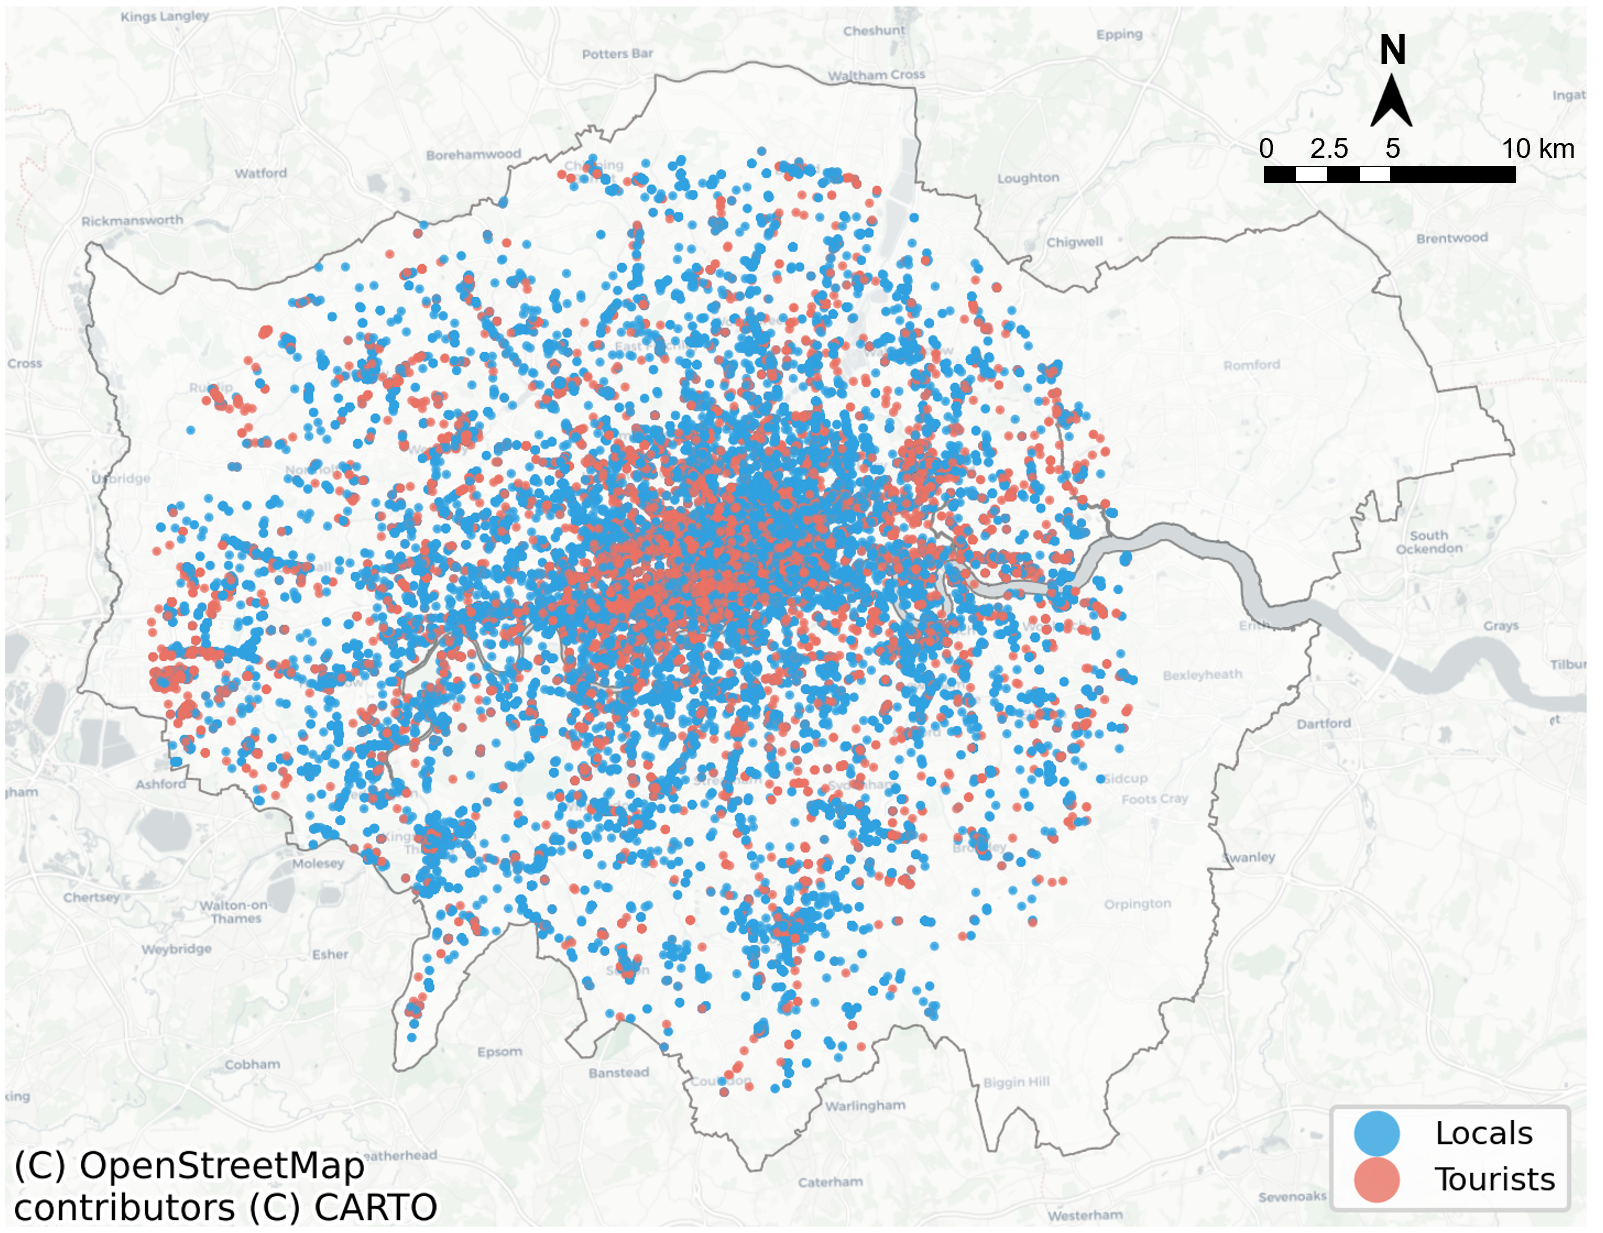
\includegraphics[width=0.7\textwidth]{figures/foursquare_distribution.png}
\caption{\label{fig:foursquare_distribution}Distribution of Foursquare check-ins of locals and tourists.}
\end{figure}

\begin{table}
\centering
\caption{\label{tab:foursquare_preprocessed}Summary of Foursquare data}
\begin{tabular}{llll} \hline
Population Group & No. of Users & No. of Check-ins\\ \hline
All Users & 7,183 & 174,609 \\
Locals & 1,087 & 108,272 \\
Tourists & 6,096 & 66,337 \\ \hline
\end{tabular}
\end{table}

For venue categories, Foursquare categorizes the place types into ten categories, namely (1) Travel \& Transport, (2) Food, (3) Professional \& Other Places, (4) Outdoors \& Recreation, (5) Shop \& Service, (6) Nightlife Spot, (7) Arts \& Entertainment, (8) College \& University, (9) Event, (10) Residence. Category 9 Event was not contained in the check-ins used in this study, and Category 10 Residence was removed to protect the privacy of users. The number of check-ins for each Foursquare venue category is shown in Table~\ref{tab:foursquare_category}. There are several combined categories in the Foursquare category system, such as Professional \& Other Places and Outdoors \& Recreation, which makes it ambiguous to determine the visiting purposes of individual check-ins. To overcome this limitation and investigate place properties more precisely, this study divided venues into 11 categories by separating the combined categories and defining new ones based on the third-level categories in the Foursquare category system. The number of check-ins for modified venue categories is presented in Table~\ref{tab:modified_category}. In terms of the category distribution among locals and tourists, the categories Transport and Restaurant were the most prevalent among both locals and tourists. However, certain categories showed a higher prevalence among a specific group, for instance, Shopping Place, Art Place, and Accommodation were more welcomed by tourists, whereas Sports Place received a greater number of check-ins from locals (Figure~\ref{fig:foursquare_category_percent}).

\begin{table}
\centering
\caption{\label{tab:foursquare_category}Foursquare venue category}
\begin{tabular}{lll} \hline
No. & Foursquare Venue Category & No. of Check-ins \\ \hline
1 & Travel \& Transport & 43,051 \\
2 & Food & 34,376 \\
3 & Professional \& Other Places & 22,184 \\
4 & Outdoors \& Recreation & 20,429 \\
5 & Shop \& Service & 19,772 \\
6 & Nightlife Spot \& Service & 18,418 \\
7 & Arts \& Entertainment & 14,285 \\
8 & College \& University & 4,692 \\ \hline
\end{tabular}
\end{table}


\begin{table}
\centering
\caption{\label{tab:modified_category}Modified Foursquare venue category}
\begin{adjustbox}{max width=\textwidth, margin=0cm}
\begin{tabular}{lllp{6cm}p{5cm}} \hline
No. & Modified Venue Category & No. of Check-ins & Foursquare Venue Category 
& Example \\ \hline
1 & Transport & 36,994 & Travel \& Transport & Airport, Train Station, Bus Station, etc. \\
2 & Restaurant & 34,376 & Food & Sandwich Place, Asian Restaurant, Italian Restaurant, etc. \\
3 & Professional Place & 29,118 & Professional \& Other Places, College \& University & Office, Government Building, Police Station, etc. \\
4 & Entertainment Place & 22,434 & Arts \& Entertainment, Shop \& Service, Nightlife Spot & Casino, Bowling Alley, Zoo, Bar, Nightclub, etc. \\
5 & Shopping Place & 18,127 & Shop \& Service & Outlet Mall, Clothing Store, Market, etc. \\
6 & Art Place & 11,132 & Arts \& Entertainment, Outdoors \& Recreation & Museum, Movie Theater, Art Gallery, Music Venue, etc. \\
7 & Green \& Blue Space & 8,220 & Outdoors \& Recreation & Park, Plaza, Garden, Lake, etc. \\
8 & Accommodation Place & 5,902 & Travel \& Transport & Hotel \\
9 & Sports Place & 5,852 & Outdoors \& Recreation & Athletics \& Sports, Pool, Playground, etc. \\
10 & Others & 3,346 & Outdoors \& Recreation, Professional \& Other Places, Travel \& Transport & Building, Bridge, Well, etc. \\
11 & Service Place & 1,706 & Travel \& Transport, Shop \& Service & Bank, Drugstore, Car Wash, Laundry Service, etc. \\ \hline
\end{tabular}
\end{adjustbox}
\end{table}

% \begin{figure}
% \centering
% 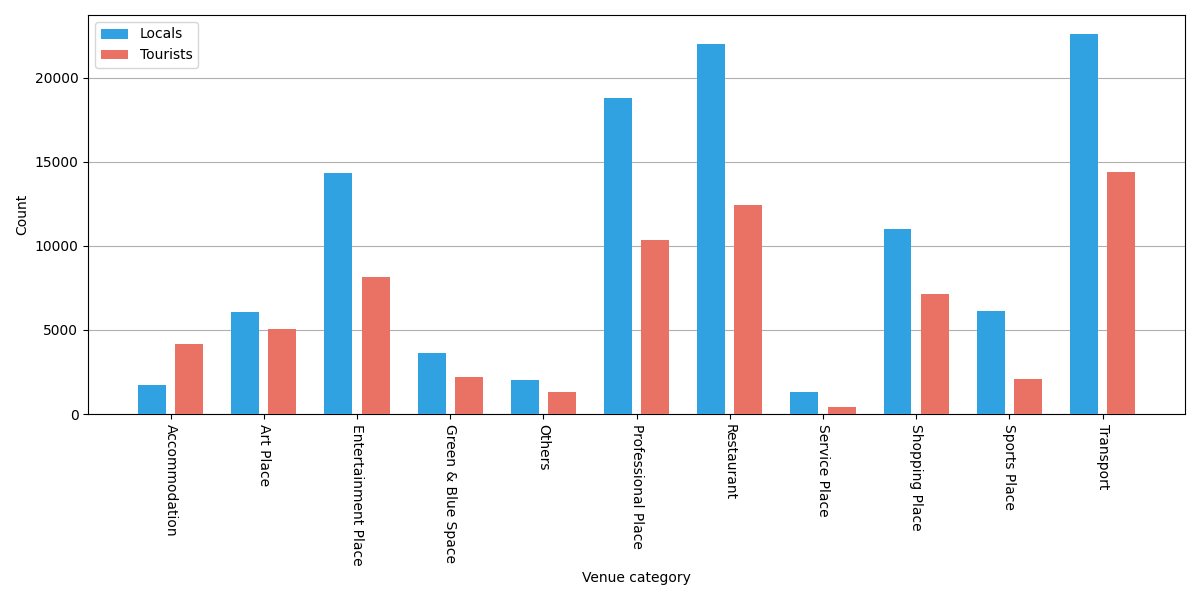
\includegraphics[width=1\textwidth]{figures/foursquare_category.png}
% \caption{\label{fig:foursquare_category}Venue categories visited by locals and tourists.}
% \end{figure}

\begin{figure}
\centering
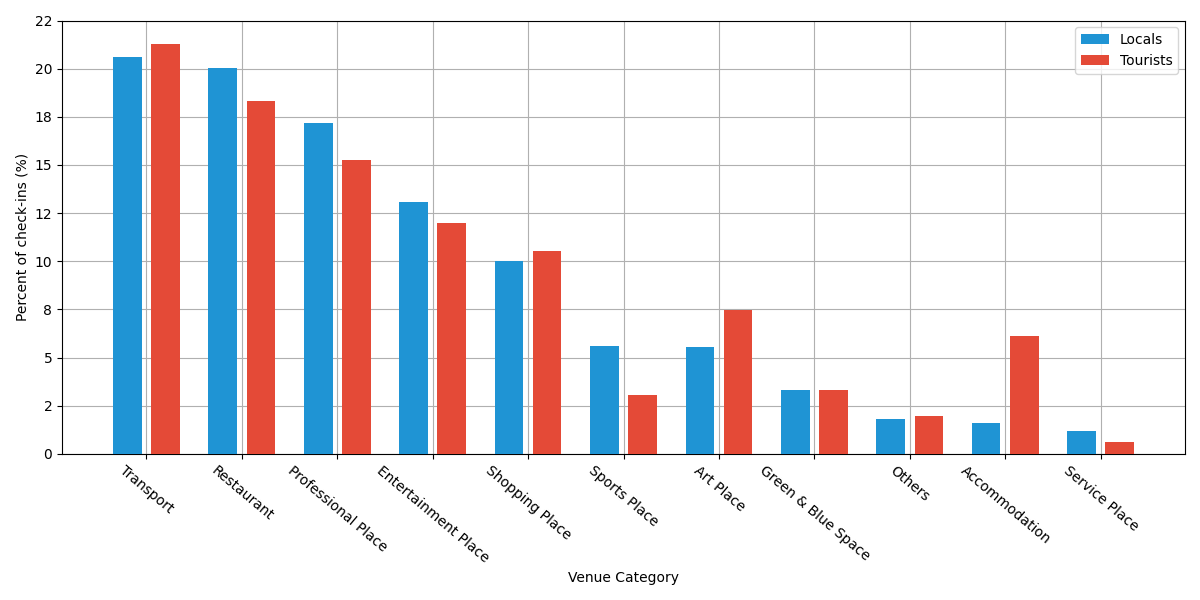
\includegraphics[width=1\textwidth]{figures/foursquare_category_percent.png}
\caption{\label{fig:foursquare_category_percent}Percent of venue categories visited by locals and tourists.}
\end{figure}



\subsubsection{Flickr Data}
Flickr is an online photo management and sharing application where users can upload photos. As of 2023, the Flickr community has shared tens of billions of photos. Flickr data was collected via \href{https://www.flickr.com/services/api/}{Flickr API} with the Python library \href{https://stuvel.eu/software/flickrapi/}{flickrapi}. To collect Flickr photos, the method \href{https://www.flickr.com/services/api/flickr.photos.search.html}{flickr.photos.search} was applied to get photos. A total of 954,260 photos with unique 250,254 tags uploaded by 28,633 users in Greater London from April 3, 2012 to September 16, 2013 were collected. The main fields of Flickr data include:
\begin{itemize}
    \item Photo ID
    \item User ID
    \item Date taken
    \item Accuracy
    \item Coordinates
    \item Tags
    \item Title
    \item Photo URL
    \item Number of views
\end{itemize}

The Flickr data required additional cleaning and identification of locals and tourists. The preprocessing steps were as follows:
\begin{enumerate}
    \item Removed photos without tags because Flickr tags were one of the main semantic information in this study.
    \item Removed photos with an accuracy level below 14. Flickr divides the accuracy level on a scale of 1 to 16, with 1 representing world-level accuracy, 2-3 representing country-level accuracy, 4-6 representing region-level accuracy, 7-11 representing city-level accuracy, and 12-16 representing street-level accuracy. Only photos with an accuracy greater than 14 were kept in this study.
    \item Removed tags that were non-Ascii characters, special characters, numbers, stop-word (e.g. a, an, the), prepositions (e.g. from, to), general place names (e.g. britain, uk, england, london), and other irrelevant tags (e.g. nikon, samsung, instagram, flickr).
    \item Removed duplicates. Duplicated tags in the same list were removed. Moreover, duplicated photos of the same user at the same location with the same tags were removed.
    \item Removed prolific and unprolific users. Prolific users were defined as those who contributed more than 5\% of all photos in the dataset, while unprolific users were defined as those who uploaded less than five photos in total per day.
    \item Removed tags with a coefficient of variation greater than 300 to reduce the contribution bias. Some tags were dominantly used by prolific users, which might lead to distortions of tags. The coefficient of variation measures whether a tag is evenly used among prolific and unprolific users \cite{hollenstein_exploring_2010}. To determine the coefficient of variation, the Flickr photos were sorted based on user contribution, with the most prolific users' photos at the top. Subsequently, all photos were equally distributed into 100 bins. For each tag, a tag profile was constructed, which stored its frequency in each of the 100 bins. The coefficient of variation was calculated as the ratio of the standard deviation to the mean of the tag frequencies in the 100 bins. The lower the coefficient of variation, the more evenly the tag is distributed. For instance, based on the histogram that displays the number of photos with a certain tag in a user distribution order, the tag \textit{square} with a coefficient of variation less than 300 is more evenly distributed than the tag \textit{forms} with a coefficient of variation greater than 300.
    \item Removed tags that were place names in Greater London. \href{http://www.geonames.org/}{GeoNames} offers \href{http://download.geonames.org/export/dump/}{Free Gazetteer Data} that includes place names in Great Britain. Place names in Greater London were filtered out from the downloaded data, and any tag that matched with these place names was removed.
    \item Identified locals and tourists based on the number of days spent in Greater London and user profiles. This study used \href{https://www.flickr.com/services/api/flickr.profile.getProfile.html}{flickr.profile.getProfile} provided by \href{https://www.flickr.com/services/api/}{Flickr API} to collect user profiles, which contained information about the users' hometowns and cities. Users who had stayed in Greater London for more than 30 days were considered locals. For the remaining users, this study would also flag them as locals if their hometown or city in their profiles was listed as London.
\end{enumerate}

After all these steps, 177,568 photos were left with a total of 717,747 tags (3,365 unique tags). These tags were used by 4,687 users, with 851 locals and 3,836 tourists uploading 259,967 and 457,780 tags respectively (Table~\ref{tab:flickr_preprocessed}). The distribution of Flickr photos indicates that the majority of photos were taken in the center of Greater London, while tourists tended to share more photos around Heathrow Airport (Figure~\ref{fig:flickr_distribution}). The word cloud in Figure~\ref{fig:flickr_tag_cloud} illustrates the most frequently used tags, including city, architecture, street, park, and art.



\begin{figure}
\centering
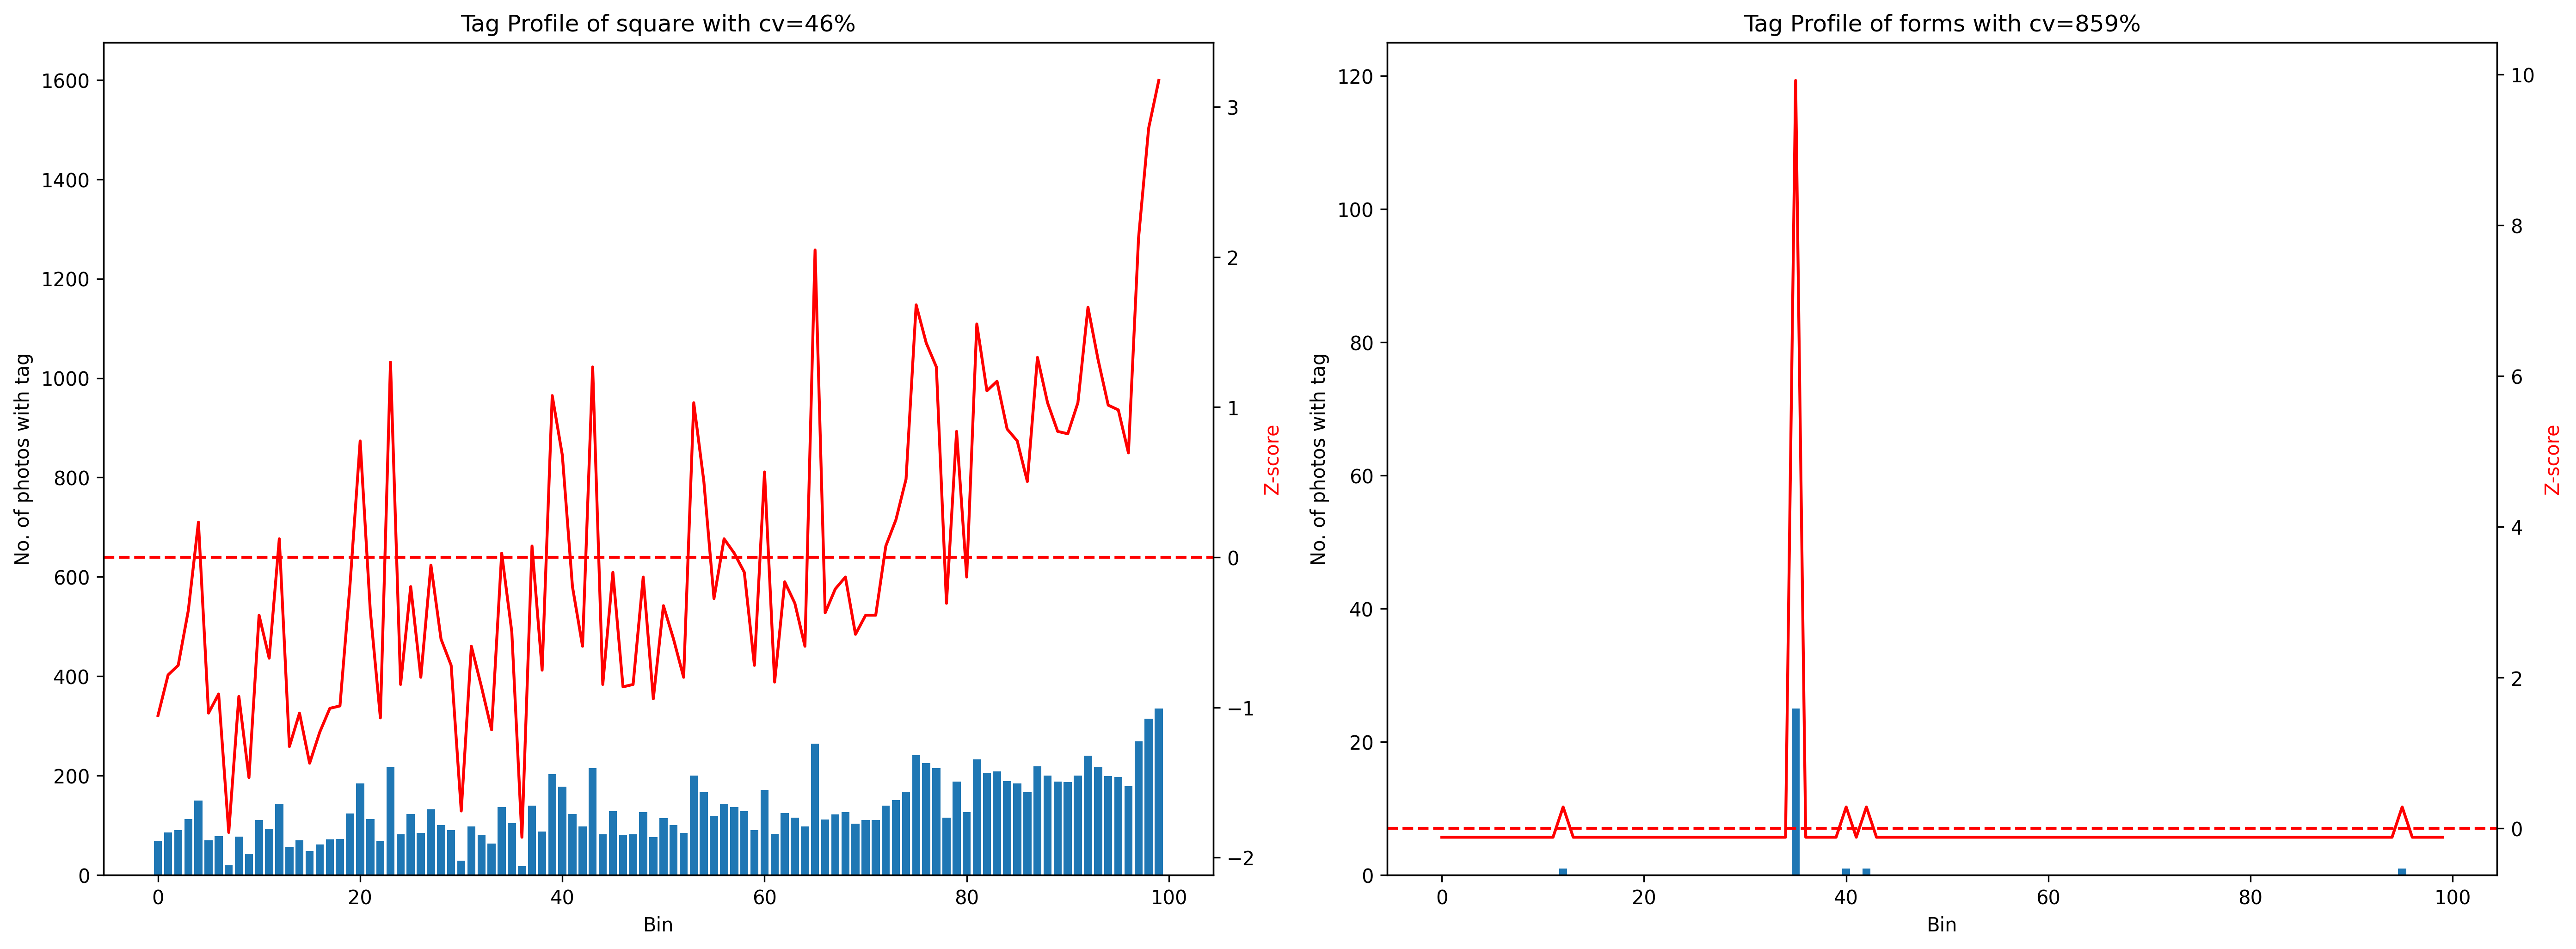
\includegraphics[width=1\textwidth]{figures/flickr_tags_cv.png}
\caption{\label{fig:flickr_tags_cv}Tag profiles.}
\end{figure}

\begin{table}
\centering
\caption{\label{tab:flickr_preprocessed}Summary of Flickr data}
\begin{tabular}{llll} \hline
Population Group & No. of Users & No. of Photos & No. of Tags \\ \hline
All Users & 4,687 & 177,568 & 717,747 \\
Locals & 851 & 65,403 & 259,967 \\
Tourists & 3,836 & 112,165 & 457,780 \\ \hline
\end{tabular}
\end{table}

\begin{figure}
\centering
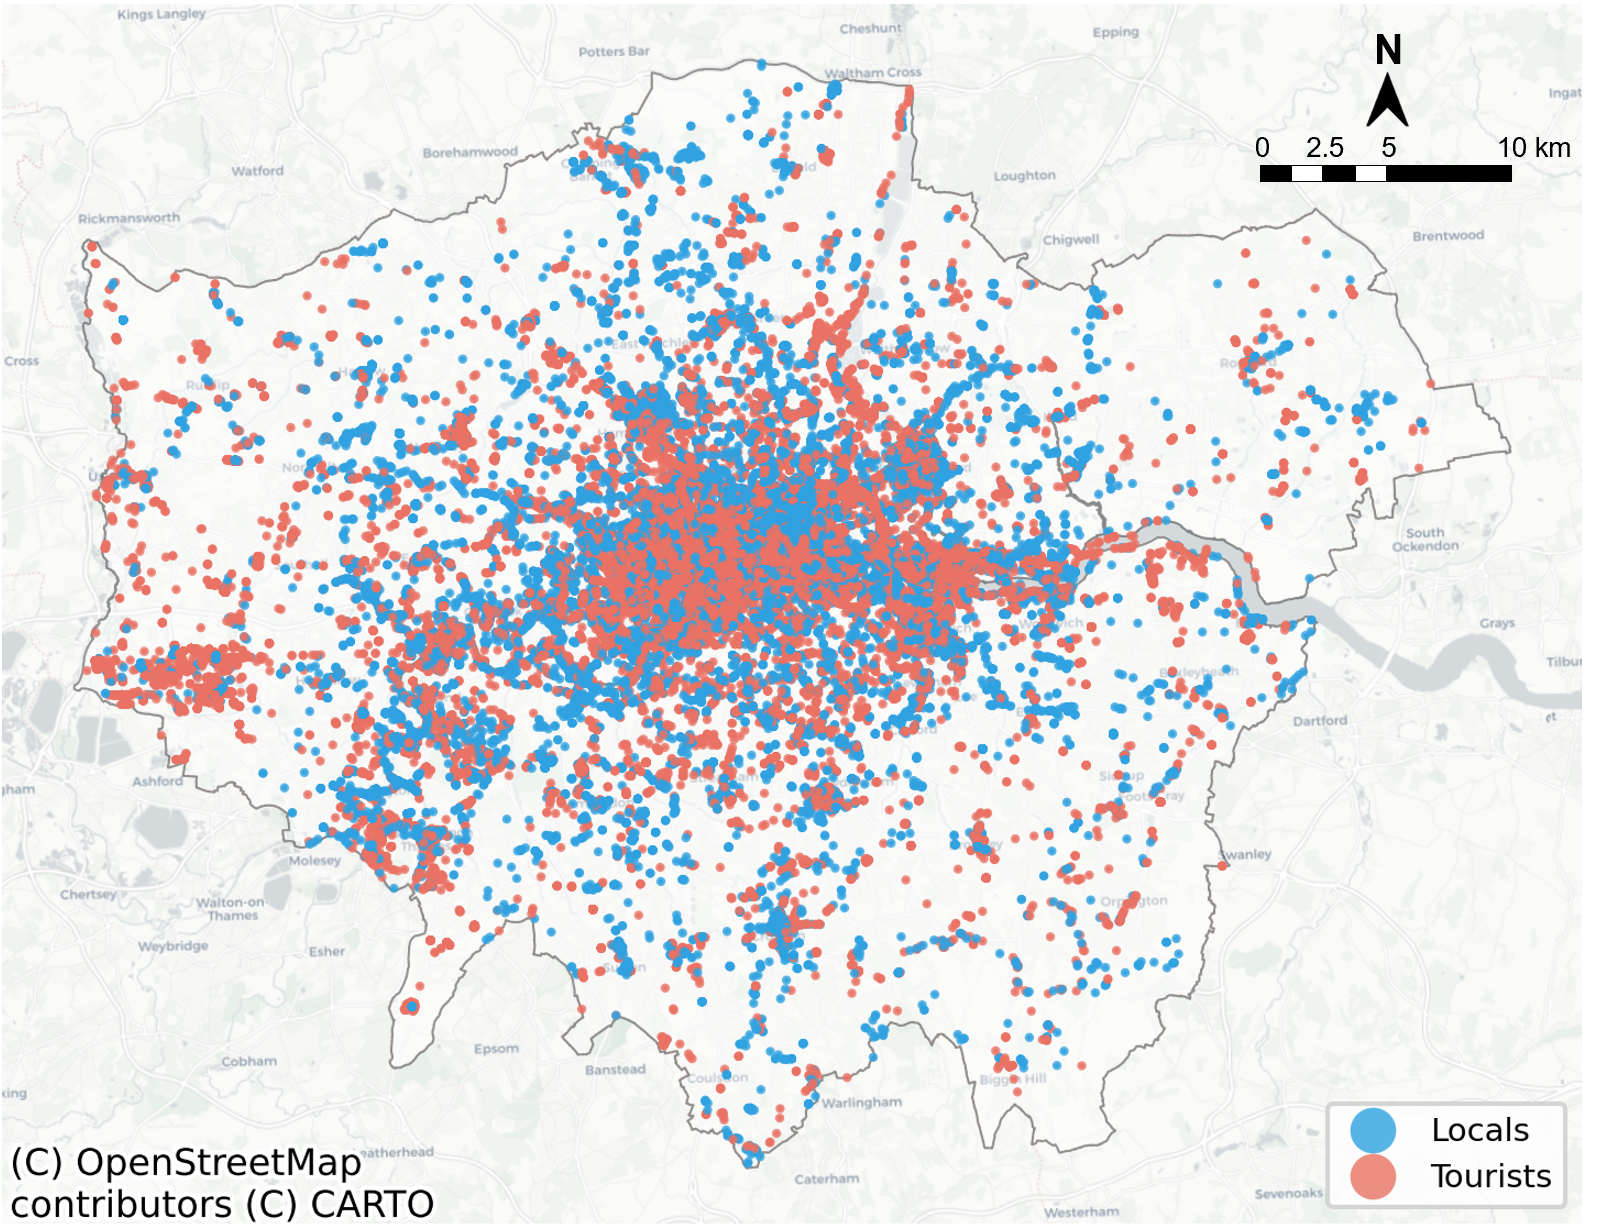
\includegraphics[width=0.7\textwidth]{figures/flickr_distribution.png}
\caption{\label{fig:flickr_distribution}Distribution of Flickr photos of locals and tourists.}
\end{figure}

\begin{figure}
\centering
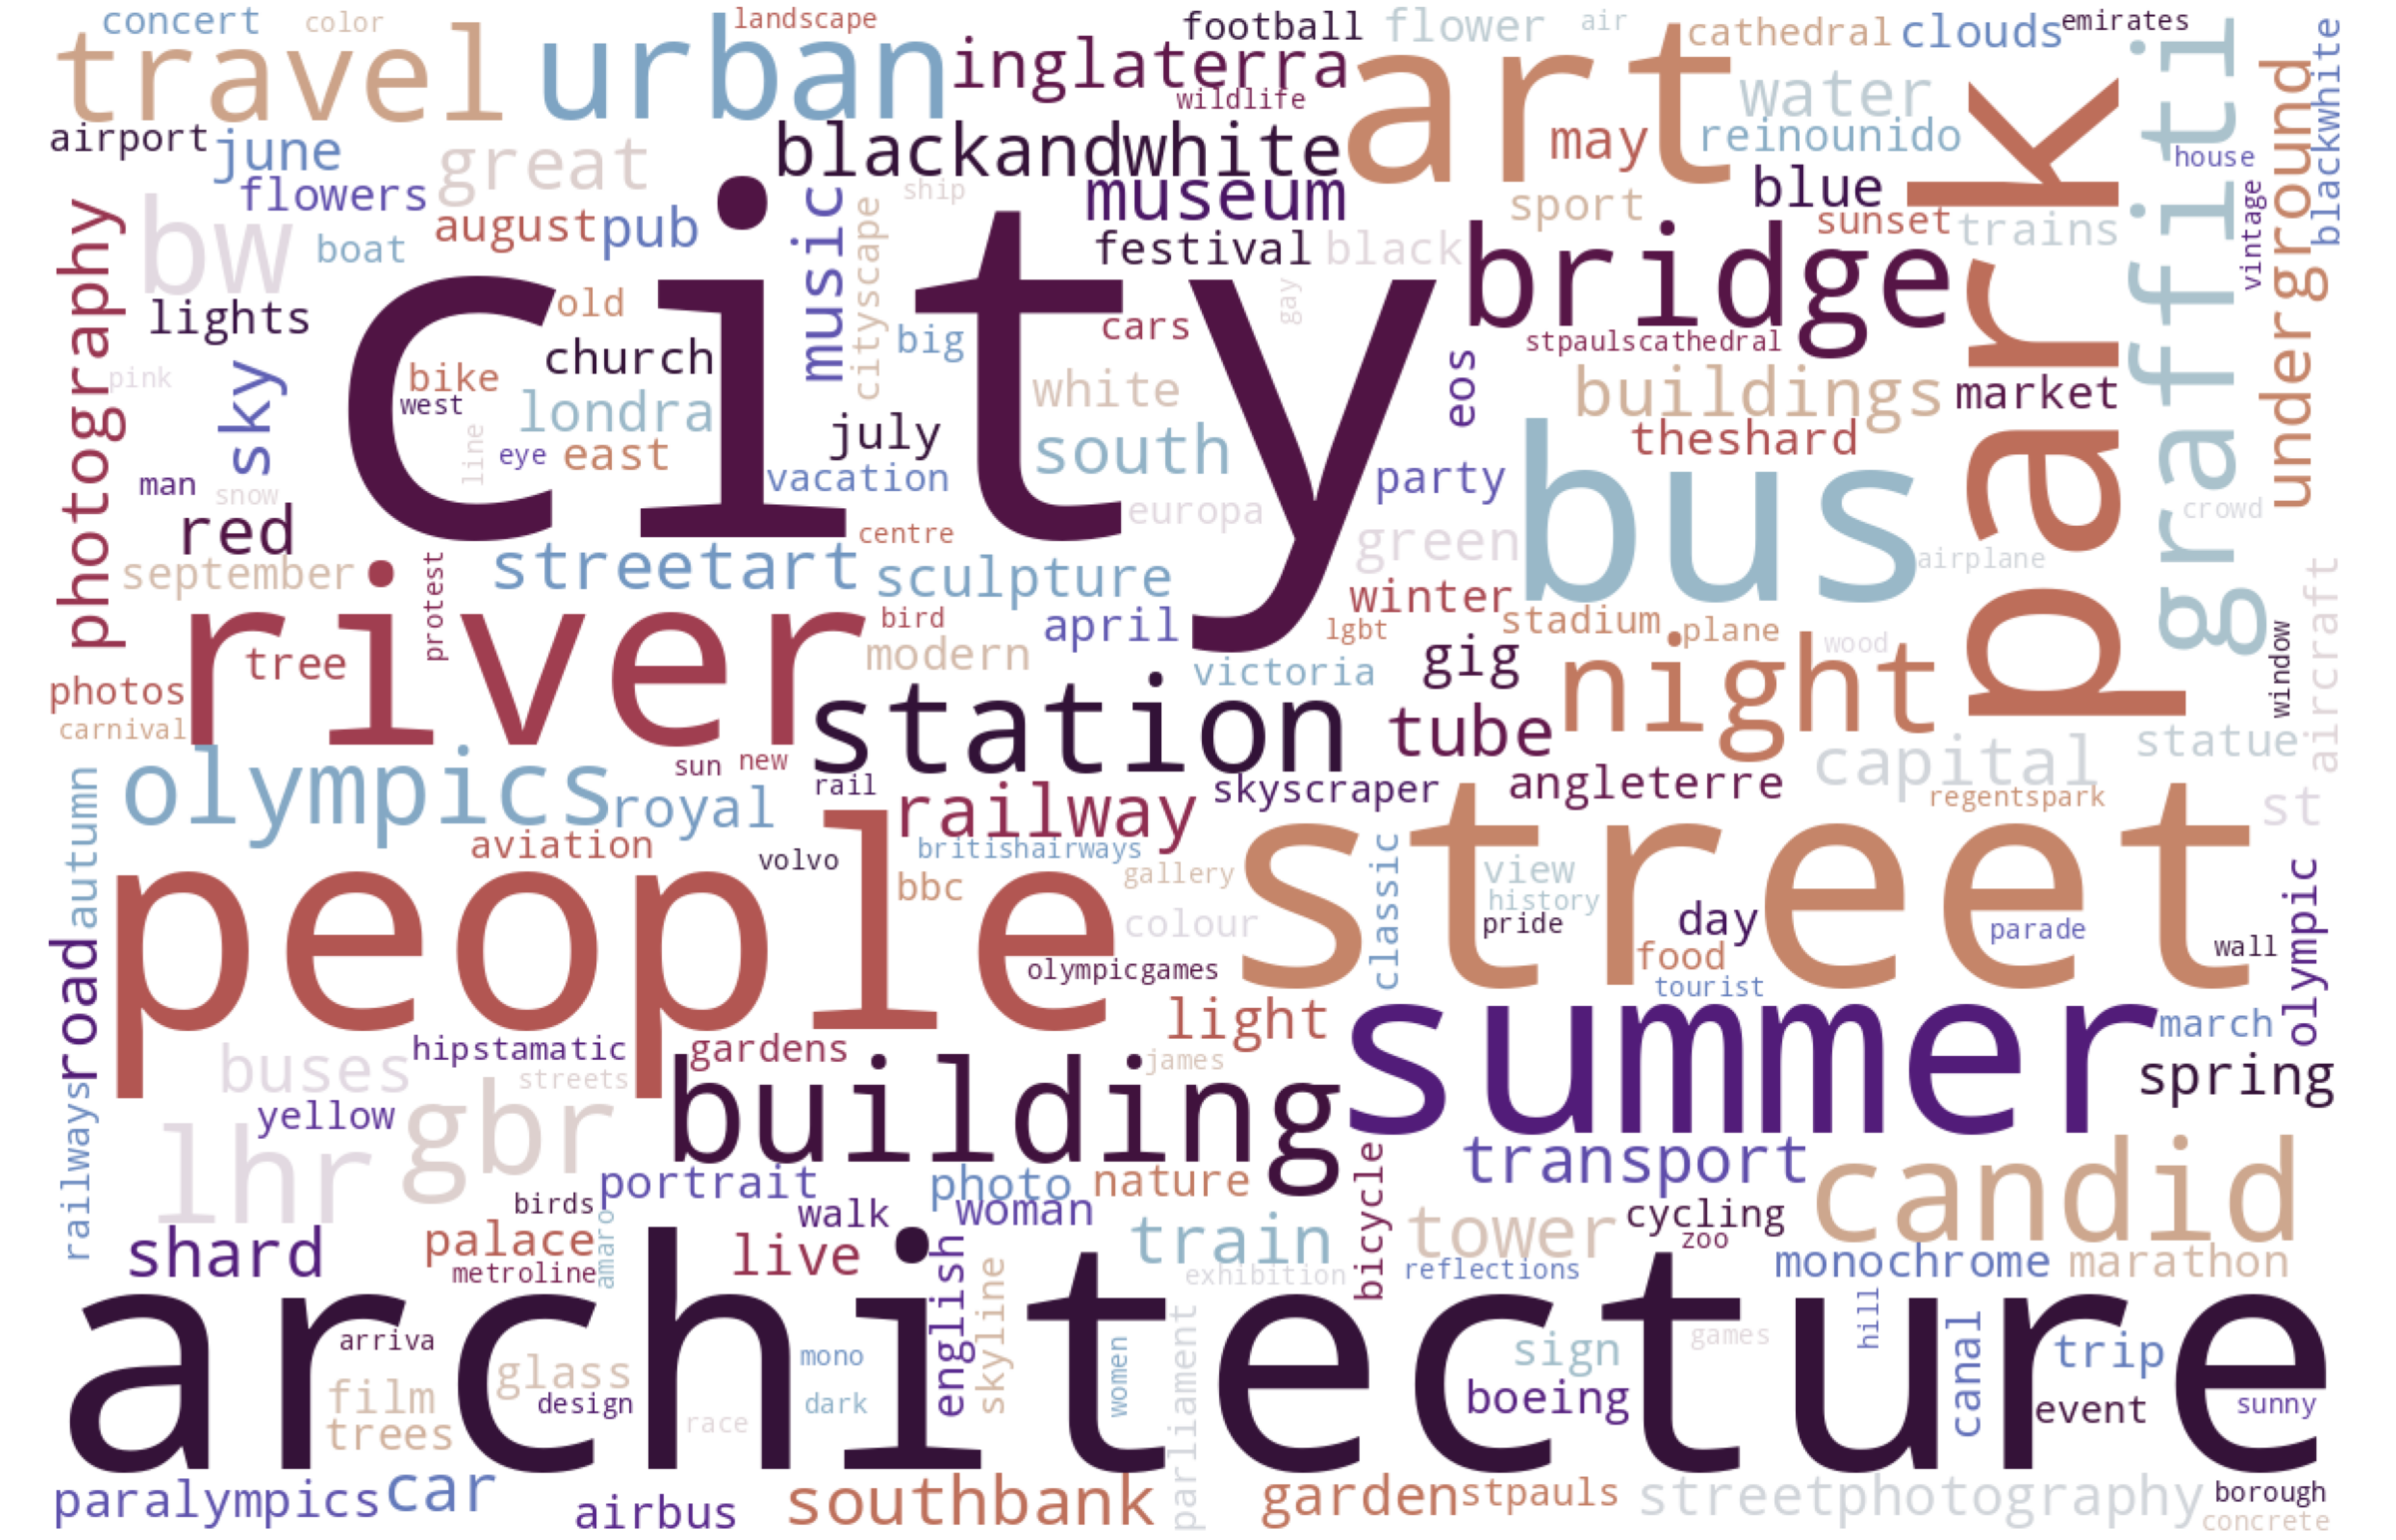
\includegraphics[width=0.7\textwidth]{figures/flickr_tag_cloud.png}
\caption{\label{fig:flickr_tag_cloud}Flickr tag cloud.}
\end{figure}


% Table~\ref{tab:popular_venues_locals}
% \begin{table}
% \centering
% \caption{\label{tab:popular_venues_locals}Top 10 popular venues for locals}
% \begin{tabular}{llll} \hline
% No. & Venue Name & No. of Check-ins & Venue Category \\ \hline
% 1 & London Waterloo Railway Station (WAT) & 874 & Transport \\
% 2 & London Paddington Railway Station (PAD) & 515 & Transport \\
% 3 & London King's Cross Railway Station (KGX) & 510 & Transport \\
% 4 & London Euston Railway Station & 463 & Transport \\
% 5 & London Victoria Railway Station (VIC) & 459 & Transport \\
% 6 & London Liverpool Street Railway Station (LST) & 407 & Transport \\
% 7 & Westfield London  & 406 & Shopping Place \\
% 8 & London Bridge Railway Station (LBG) & 366 & Transport \\
% 9 & Westfield Stratford City & 353 & Shopping Place \\
% 10 & London St Pancras International Railway Station (STP) & 302 & Transport \\ \hline
% \end{tabular}
% \end{table}

% Table~\ref{tab:popular_venues_tourists}
% \begin{table}
% \centering
% \caption{\label{tab:popular_venues_tourists}Top 10 popular venues for tourists}
% \begin{tabular}{llll} \hline
% No. & Venue Name & No. of Check-ins & Venue Category \\ \hline
% 1 & London Euston Railway Station & 944 & Transport \\
% 2 & London King's Cross Railway Station (KGX) & 693 & Transport \\
% 3 & London Paddington Railway Station (PAD) & 616 & Transport \\
% 4 & Harrods & 610 & Shopping Place \\
% 5 & London Waterloo Railway Station (WAT) & 587 & Transport \\
% 6 & London Victoria Railway Station (VIC) & 493 & Transport \\
% 7 & London St Pancras International Railway Station (STP) & 489 & Transport \\
% 8 & Piccadilly Circus & 468 & Green \& Blue Space \\
% 9 & Buckingham Palace & 440 & Art Place \\
% 10 & Trafalgar Square & 397 & Green \& Blue Space \\ \hline
% \end{tabular}
% \end{table}

% Table~\ref{tab:popular_venues_daytime_locals}
% \begin{table}
% \centering
% \caption{\label{tab:popular_venues_daytime_locals}Top 10 popular venues for locals during daytime}
% \begin{tabular}{llll} \hline
% No. & Venue Name & No. of Check-ins & Venue Category \\ \hline
% 1 & London Waterloo Railway Station (WAT) & 723 & Transport \\
% 2 & London Paddington Railway Station (PAD) & 439 & Transport \\
% 3 & London King's Cross Railway Station (KGX) & 427 & Transport \\
% 4 & London Euston Railway Station & 397 & Transport \\
% 5 & London Victoria Railway Station (VIC) & 397 & Transport \\
% 6 & London Liverpool Street Railway Station (LST) & 351 & Transport \\
% 7 & Westfield London & 343 & Shopping Place \\
% 8 & Westfield Stratford City & 314 & Shopping Place \\
% 9 & London Bridge Railway Station (LBG) & 301 & Transport \\
% 10 & London St Pancras International Railway Station (STP) & 252 & Transport \\ \hline
% \end{tabular}
% \end{table}
\newpage


\section{Methodology}
\underline{refer to notes in logbooks!!!!}

\underline{pseudocode}

\underline{Figure~\ref{fig:flowchart}}
\begin{figure}
\centering
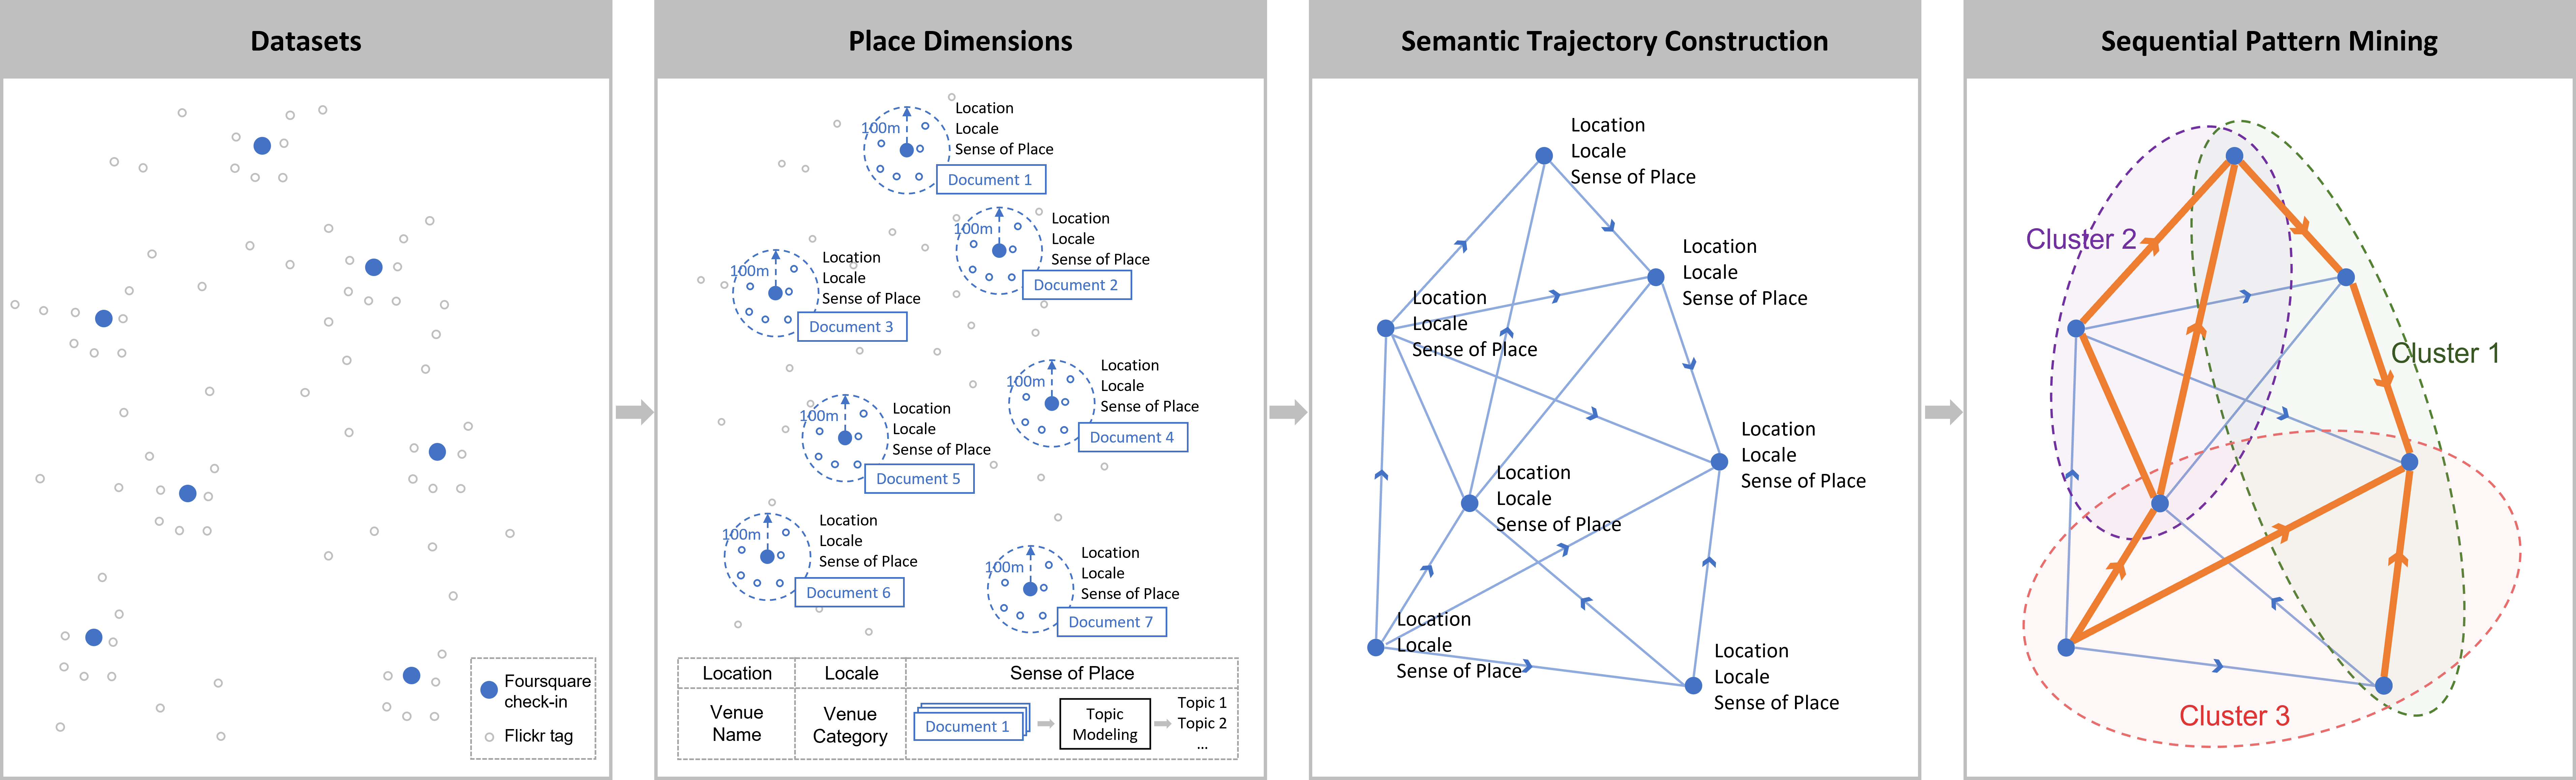
\includegraphics[width=1\textwidth]{figures/flowchart.png}
\caption{\label{fig:flowchart}Flickr tag cloud.}
\end{figure}

\subsection{Place Distribution}
\subsubsection{Preferences of Locals and Tourists}
Difference ratio

Explain why a comparison should be made, and which approach was applied (formula for Difference ratio)

top-ranked locations, location importance: \cite{yin_diversified_2011}

\subsubsection{Place Clustering}
K-means

\subsection{Place Dimensions}
\subsubsection{Definition of Dimensions}
Location, Locale, Sense of Place
% however, the identity of the place should also be considered in the definition of place, as it distinguishes place from location. Compared with location, which is merely a point described by coordinates, place is an identifiable location formed based on human consensus with definable properties \citep{purves_places_2019}.

sense of place:
People's emotional relationships with places are subjective and need not be strong and positive \citep{altman_place_1992}. Someone may feel nostalgic about the place he used to visit, even if the place itself is not objectively positive or negative \cite{relph_geographical_1985}. Descriptive words can also be used to describe emotions about a place other than simply positive or negative.

\subsubsection{Topic Modeling}
introduction to topic modeling, topic modeling formula, gensim, pyLDAvis

Concept talk question: Buffer overlap of Foursquare places, which makes the same Flickr tag belongs to two places

LDAcvis

\subsection{Semantic Trajectories Patterns}
introduce the process
\cite{alvares_model_2007}

\subsubsection{Exploratory Analysis???}

\subsubsection{Trajectories Construction}
cite trajminer

remove check-ins in trajectories with length less than 3 >>> topic modeling >>> trajectory construction

Foursquare check-ins with no nearby Flickr tags >>>
Tried buffer sizes of 1000m, 500m, and 250m, but there are always check-ins with no Flickr tags around >>>
Applied the topic imputation for these check-ins >>>
Gaussian kernel >>>
Buffer size of 500m has the best coherence value in topic modeling

\subsubsection{Trajectories Similarity}
MSM, MUITAS
\subsubsection{Trajectories Clustering}
Agglomerative Clustering, DBSCAN

\underline{Concept talk question: Locals and tourists have very different trajectories, how to compare them?

(1) Describe what the trajectories of locals and tourists look like, and what’s the visiting direction

(2) Make histograms about the main place types and topics within the trajectories, and compare them

https://www.tandfonline.com/doi/full/10.1080/15481603.2021.1908927}
\newpage

\subsection{Results Evaluation???}


\section{Results}
\subsection{Functionalities of Places}
\subsubsection{Daytime vs. Nighttime}
\subsubsection{Weekday vs. Weekend}

\subsection{topic modeling}

\subsection{semantic trajectories/city perception}
\subsubsection{Daytime vs. Nighttime}
\subsubsection{Weekday vs. Weekend}

RQ1: What’s the functionality of the place based on the visit number of locals and tourists?

For each section,
include tables on the number of locals and tourists during daytime, nighttime/weekday, weekend

include tables and figures on the visiting frequencies to foursquare check-ins category of locals and tourists, and briefly describe which categories are more frequently visited by locals/tourists
% https://colab.research.google.com/drive/1xLXGgWscXJIaRYVmw7RzFpymd2js7Kuc#scrollTo=8aQpz87SLvQQ


Figure \ref{fig:foursquare_day_count_pie}
\begin{figure}
\centering
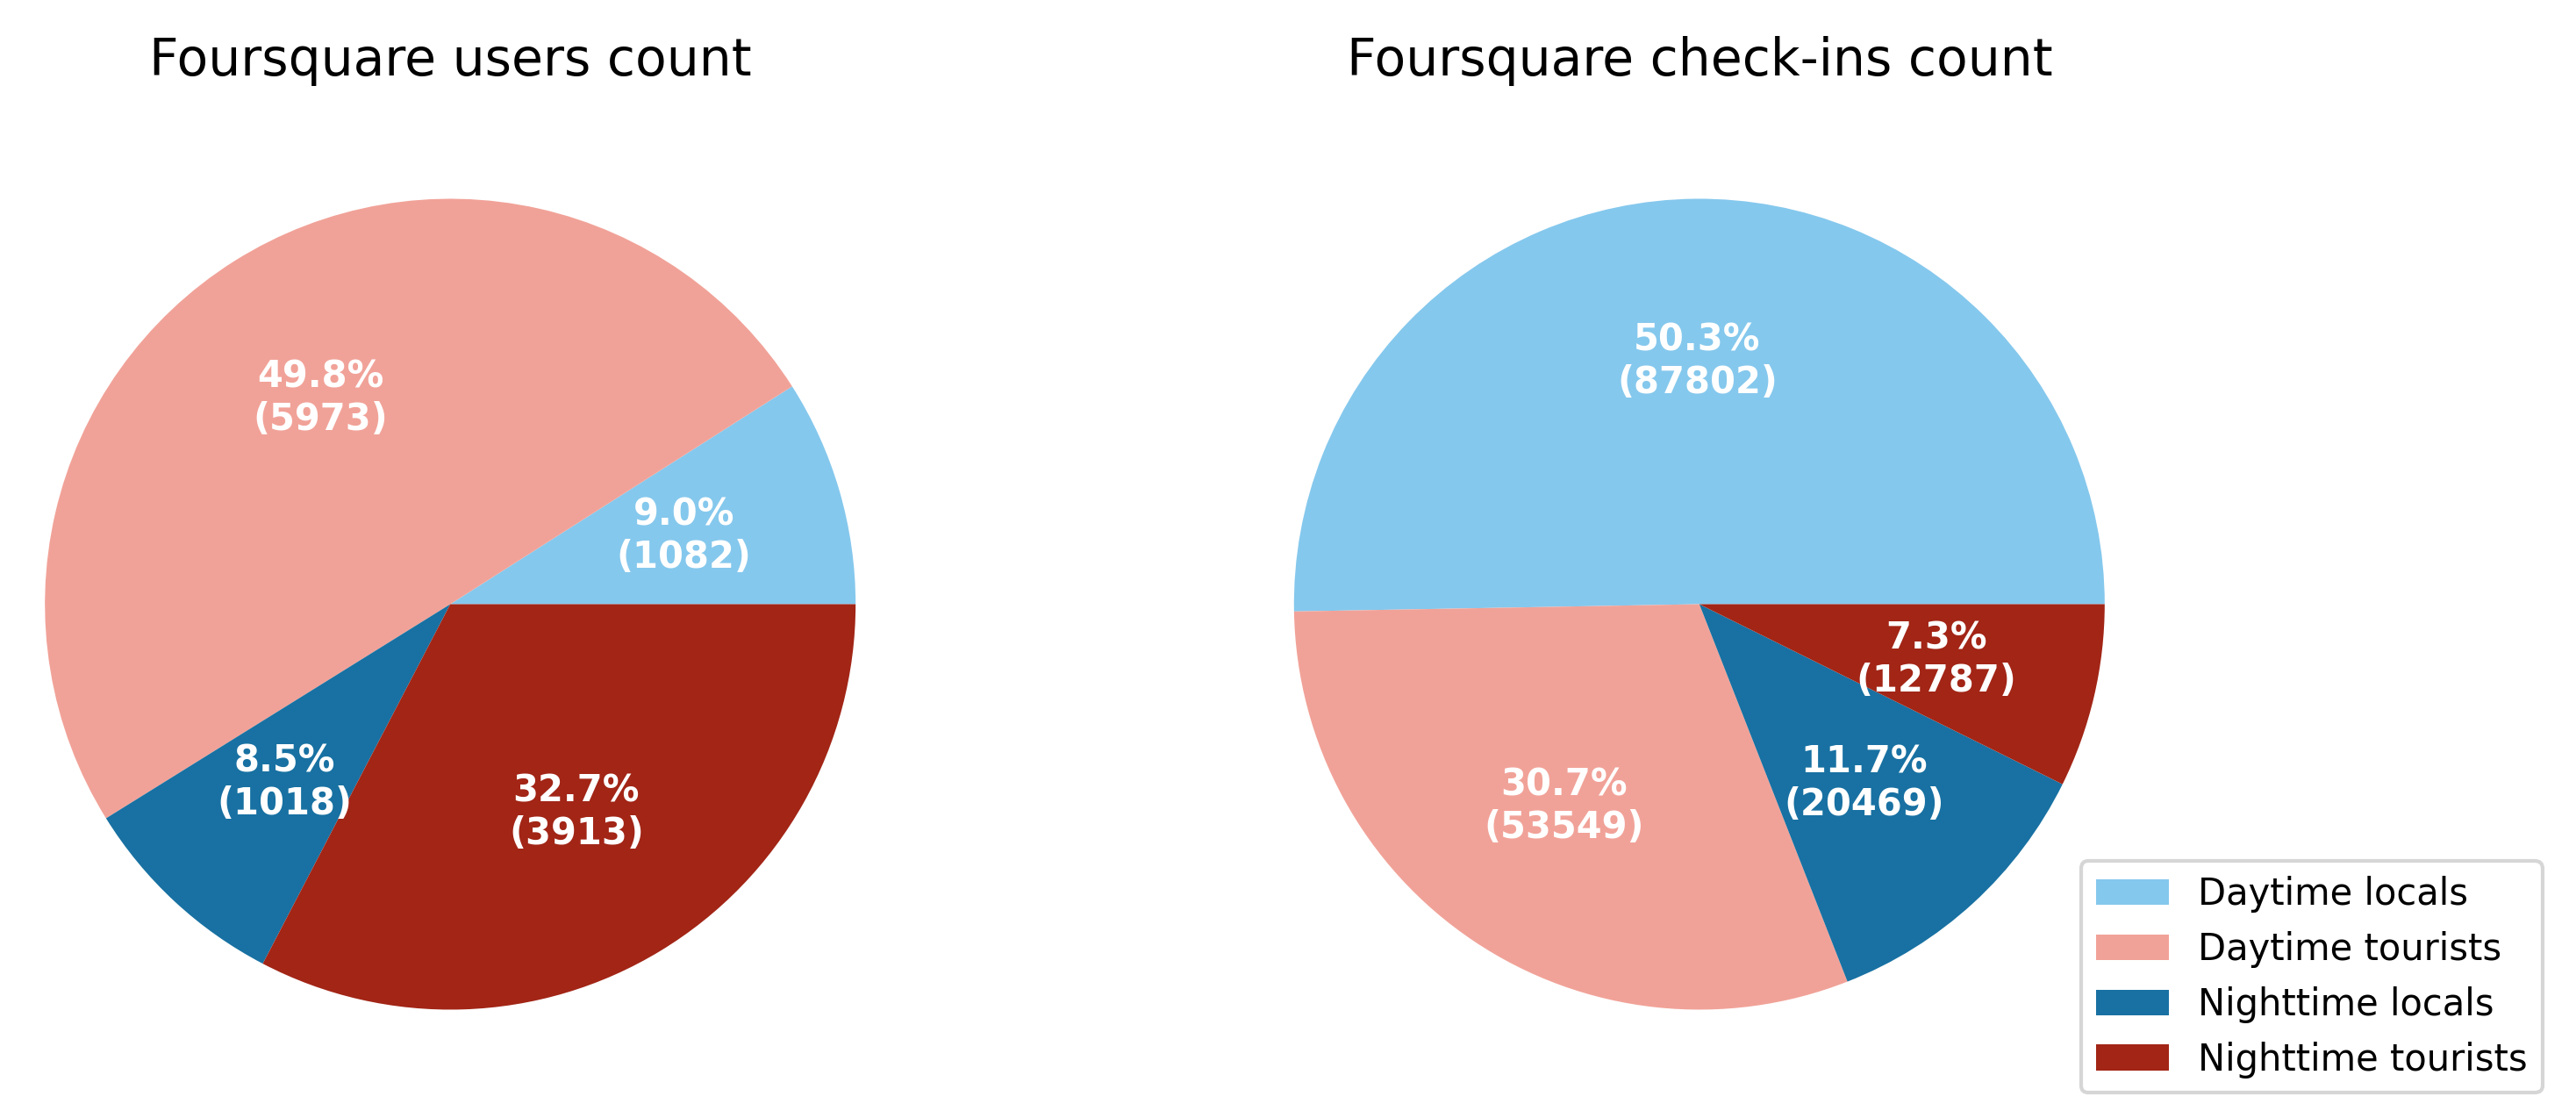
\includegraphics[width=0.75\textwidth]{figures/foursquare_day_count_pie.png}
\caption{\label{fig:foursquare_day_count_pie}Percent of Foursquare data of locals and tourists during daytime and nighttime.}
\end{figure}

Figure \ref{fig:flickr_day_count_pie}
\begin{figure}
\centering
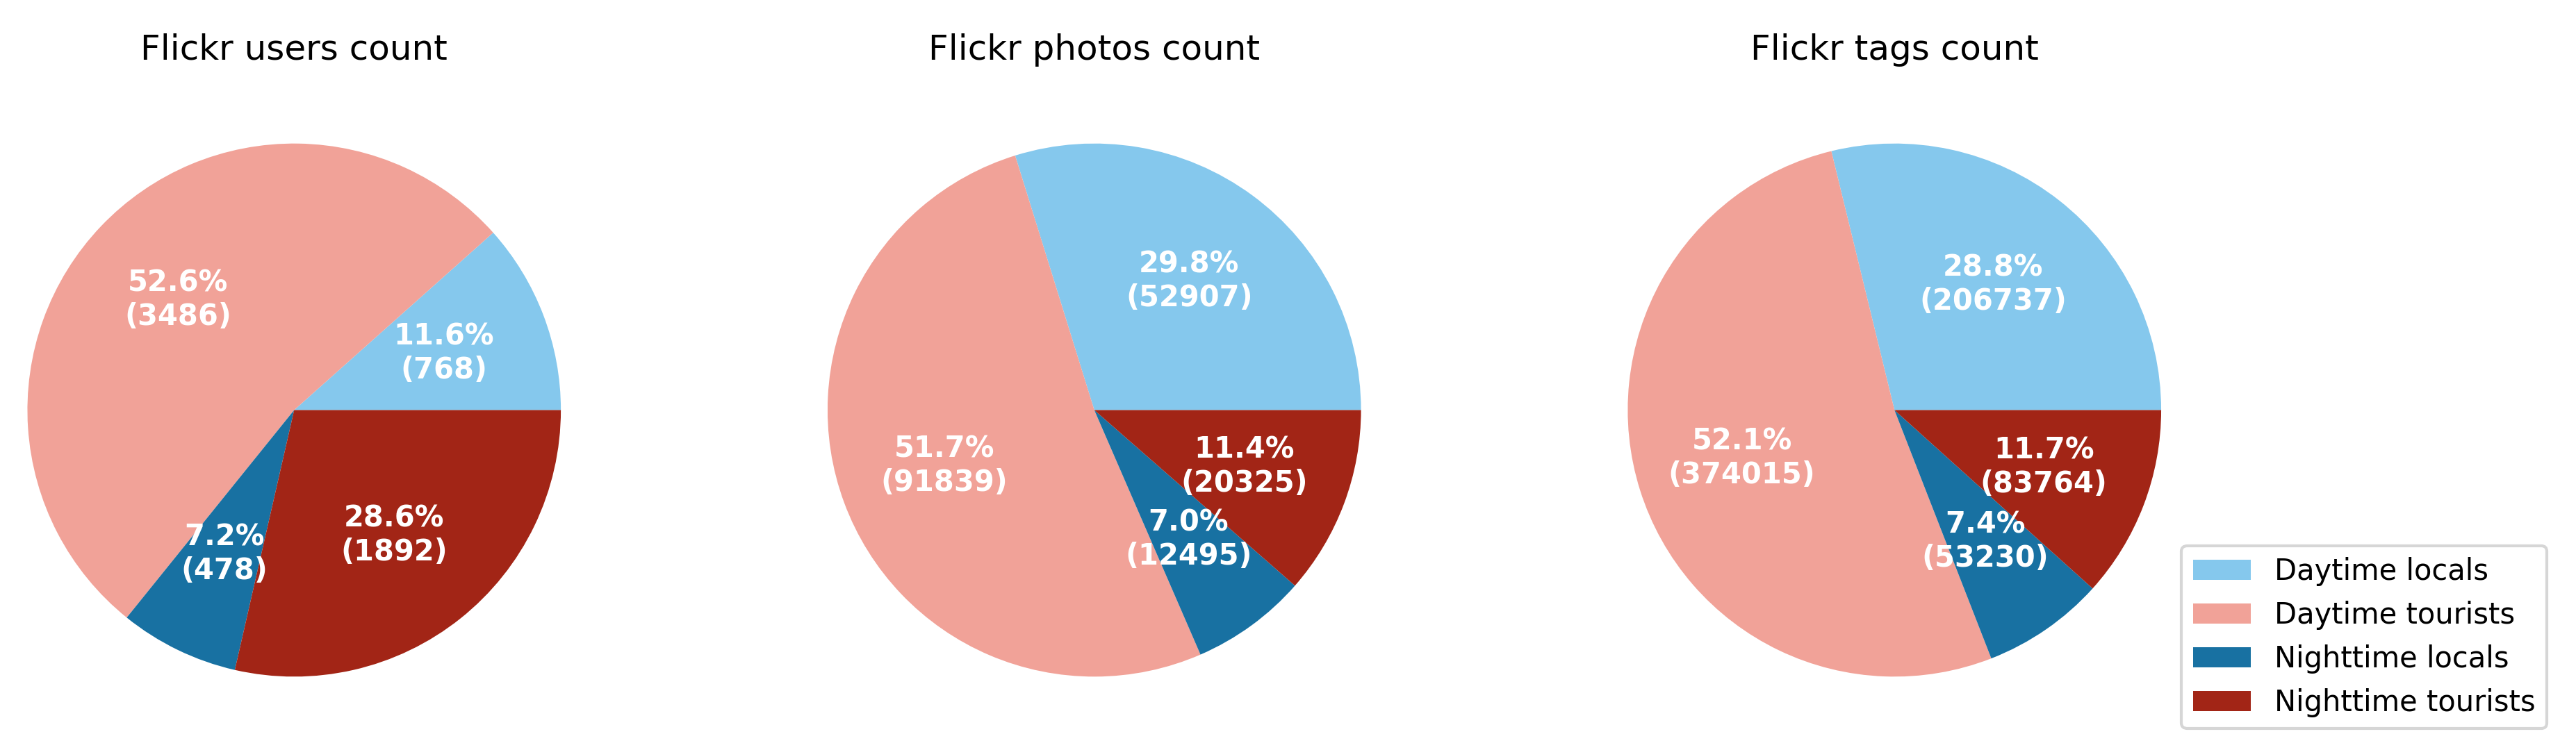
\includegraphics[width=1.13\textwidth]{figures/flickr_day_count_pie.png}
\caption{\label{fig:flickr_day_count_pie}Percent of Flickr data of locals and tourists during daytime and nighttime.}
\end{figure}


Figure \ref{fig:foursquare_week_count_pie}
\begin{figure}
\centering
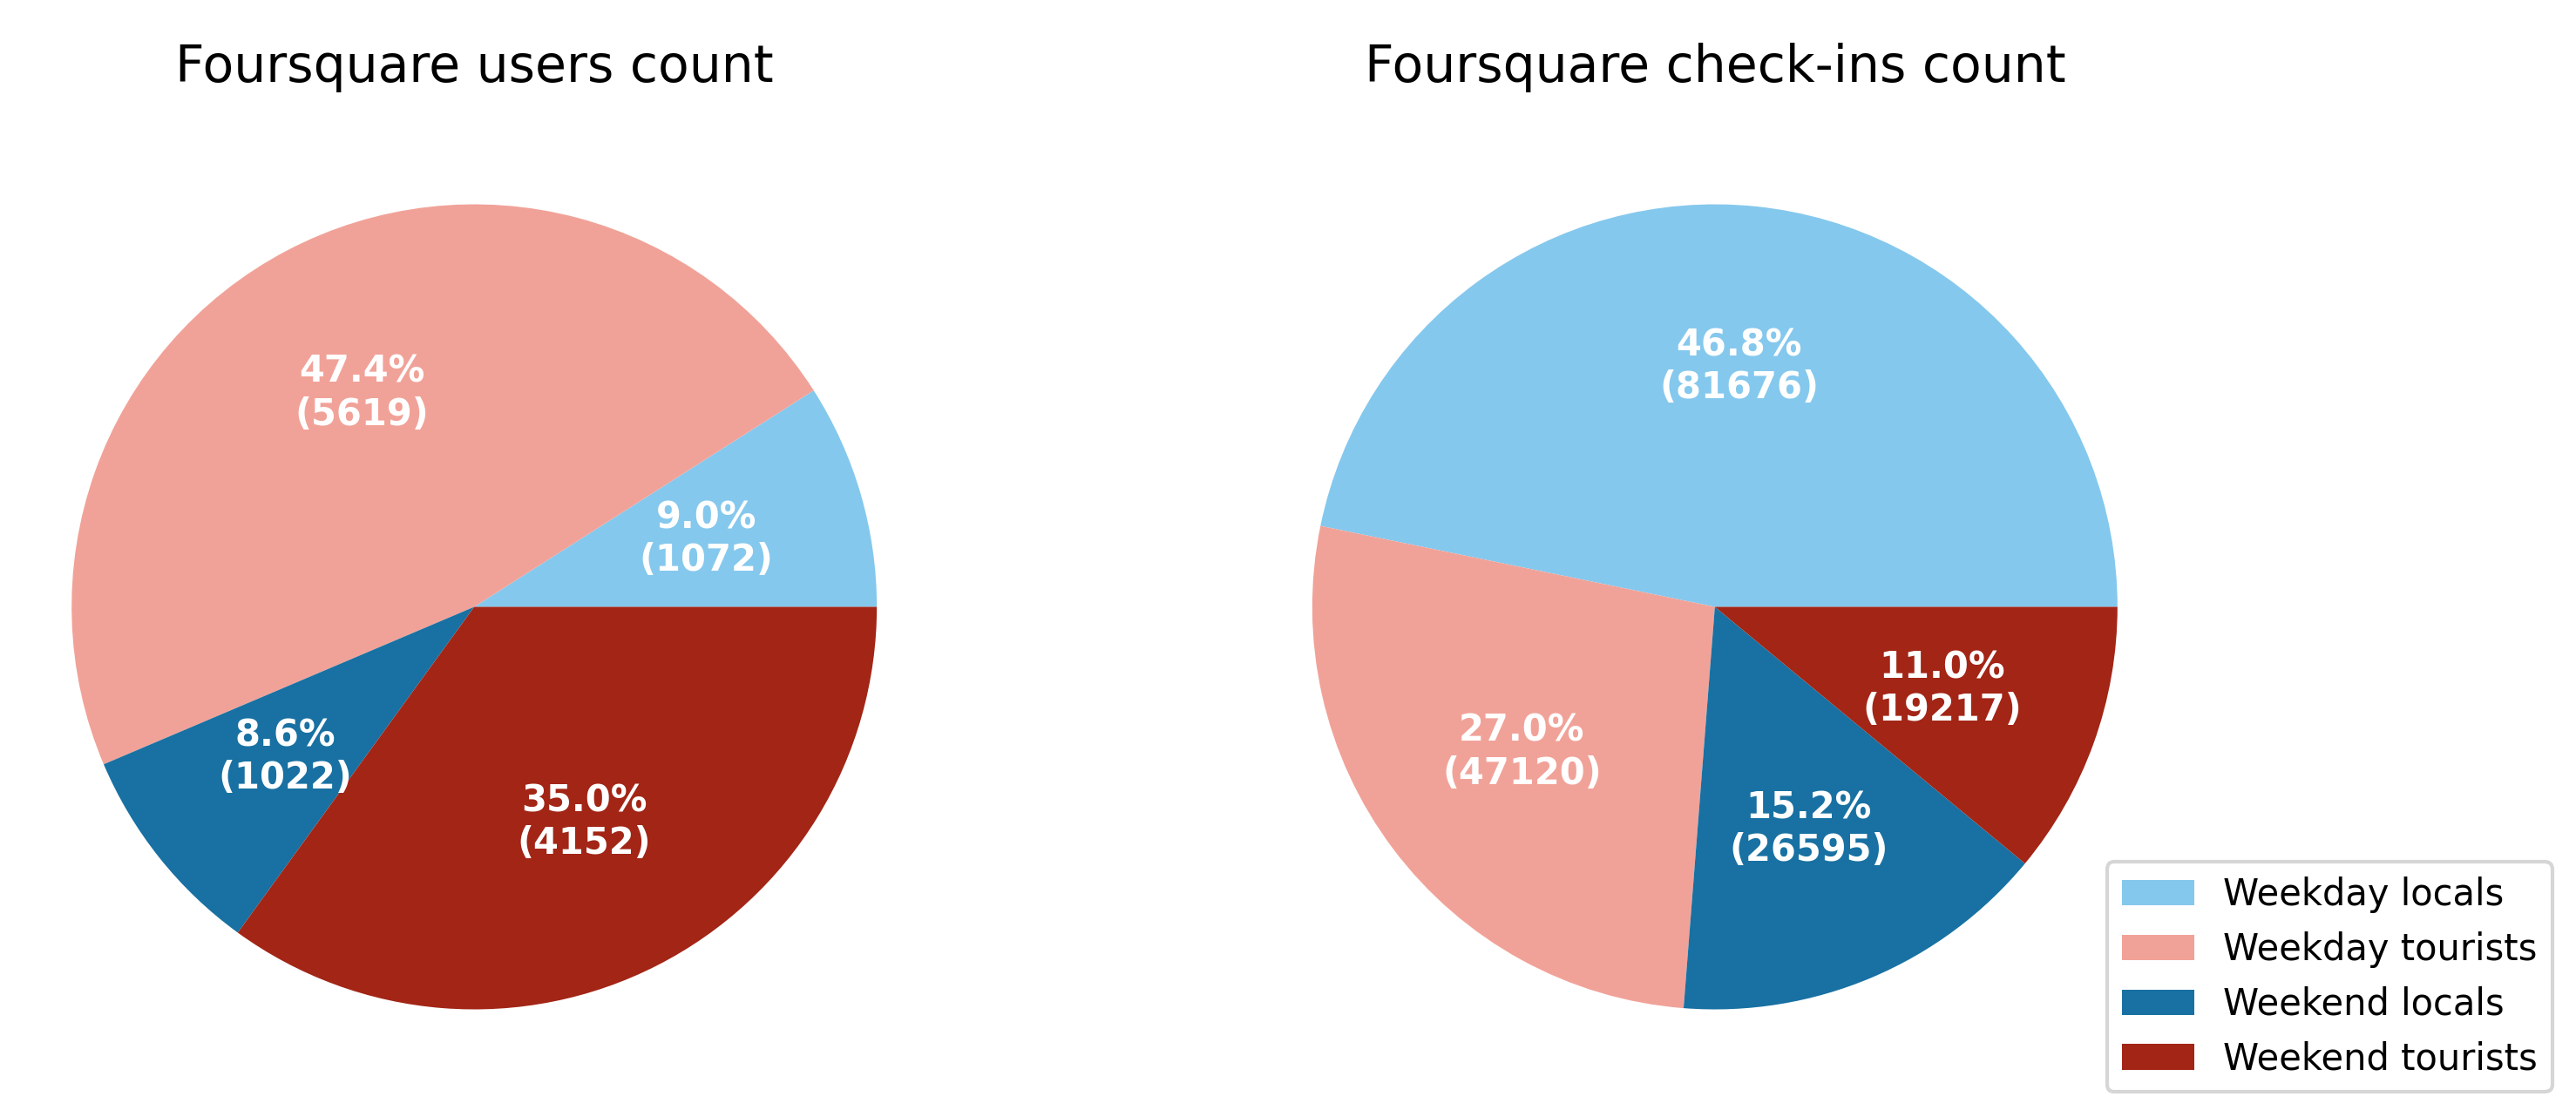
\includegraphics[width=0.75\textwidth]{figures/foursquare_week_count_pie.png}
\caption{\label{fig:foursquare_week_count_pie}Percent of Foursquare data of locals and tourists during weekdays and weekends.}
\end{figure}

Figure \ref{fig:flickr_week_count_pie}
\begin{figure}
\centering
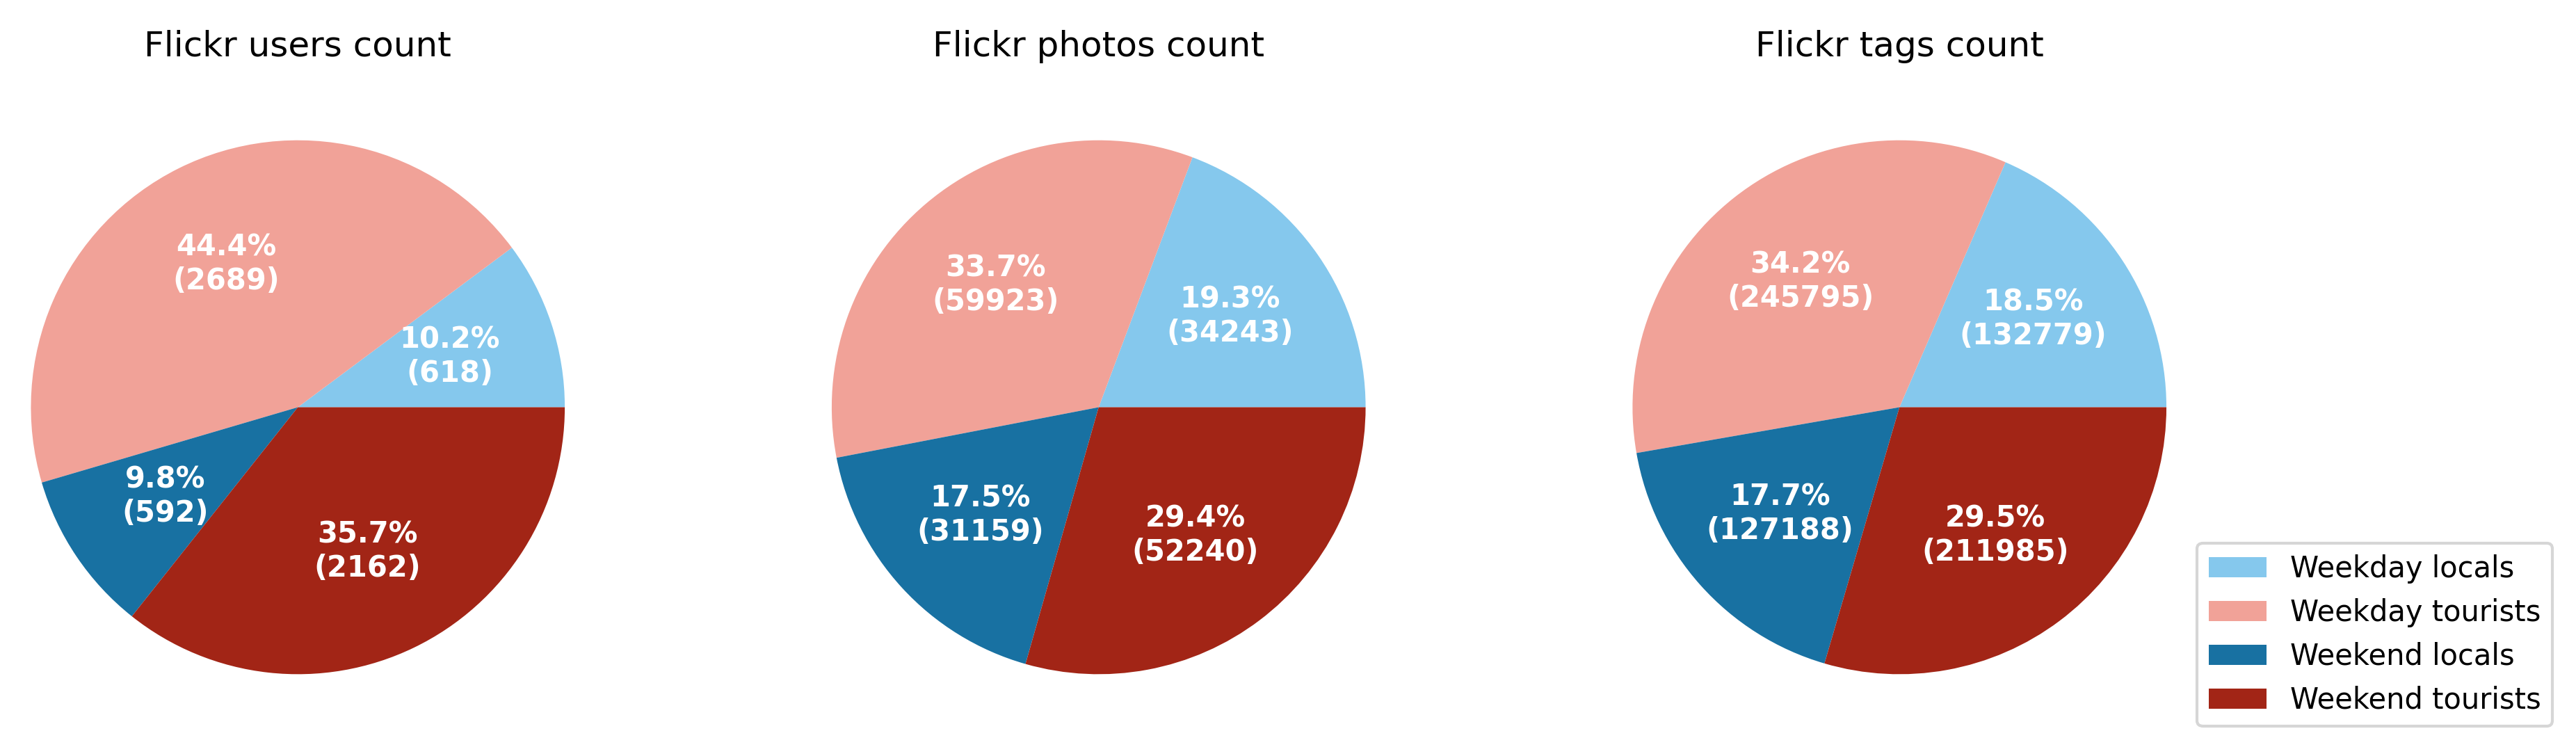
\includegraphics[width=1.13\textwidth]{figures/flickr_week_count_pie.png}
\caption{\label{fig:flickr_week_count_pie}Percent of Flickr data of locals and tourists during weekdays and weekends.}
\end{figure}


RQ2: How do locals and tourists perceive the city along their semantic trajectories at different time spans

Figure \ref{fig:foursquare_trend_day}
\begin{figure}
\centering
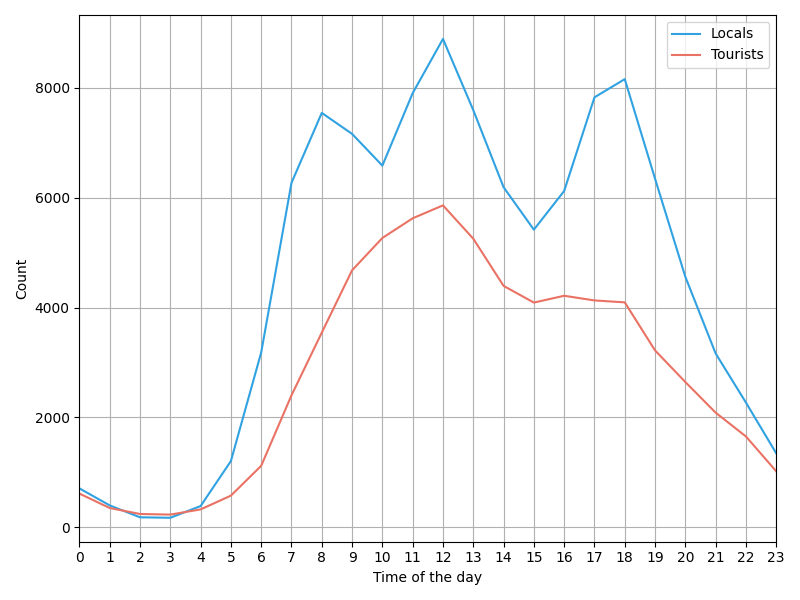
\includegraphics[width=0.8\textwidth]{figures/foursquare_trend_day.png}
\caption{\label{fig:foursquare_trend_day}Temporal Foursquare check-ins sharing pattern along the day.}
\end{figure}

Figure \ref{fig:foursquare_trend_week}
\begin{figure}
\centering
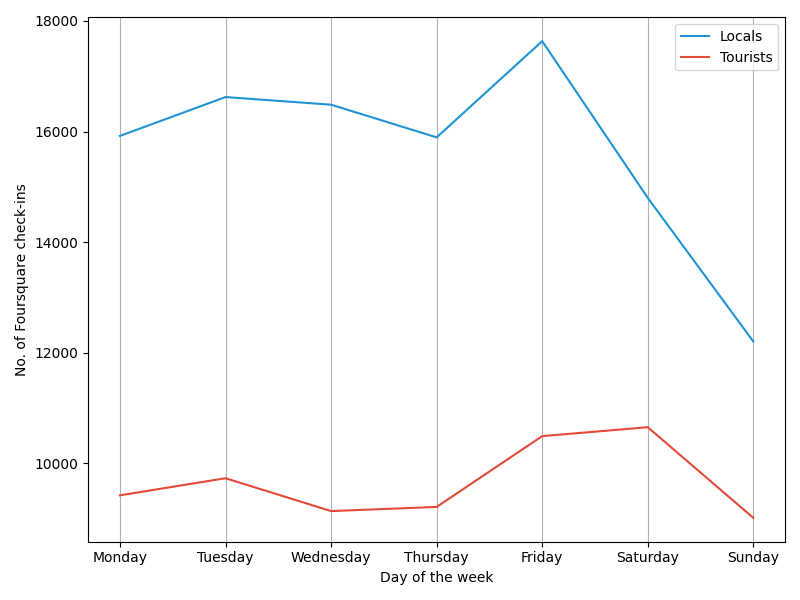
\includegraphics[width=0.8\textwidth]{figures/foursquare_trend_week.png}
\caption{\label{fig:foursquare_trend_week}Temporal Foursquare check-ins sharing pattern along the week.}
\end{figure}


Figure \ref{fig:flickr_trend_day}
\begin{figure}
\centering
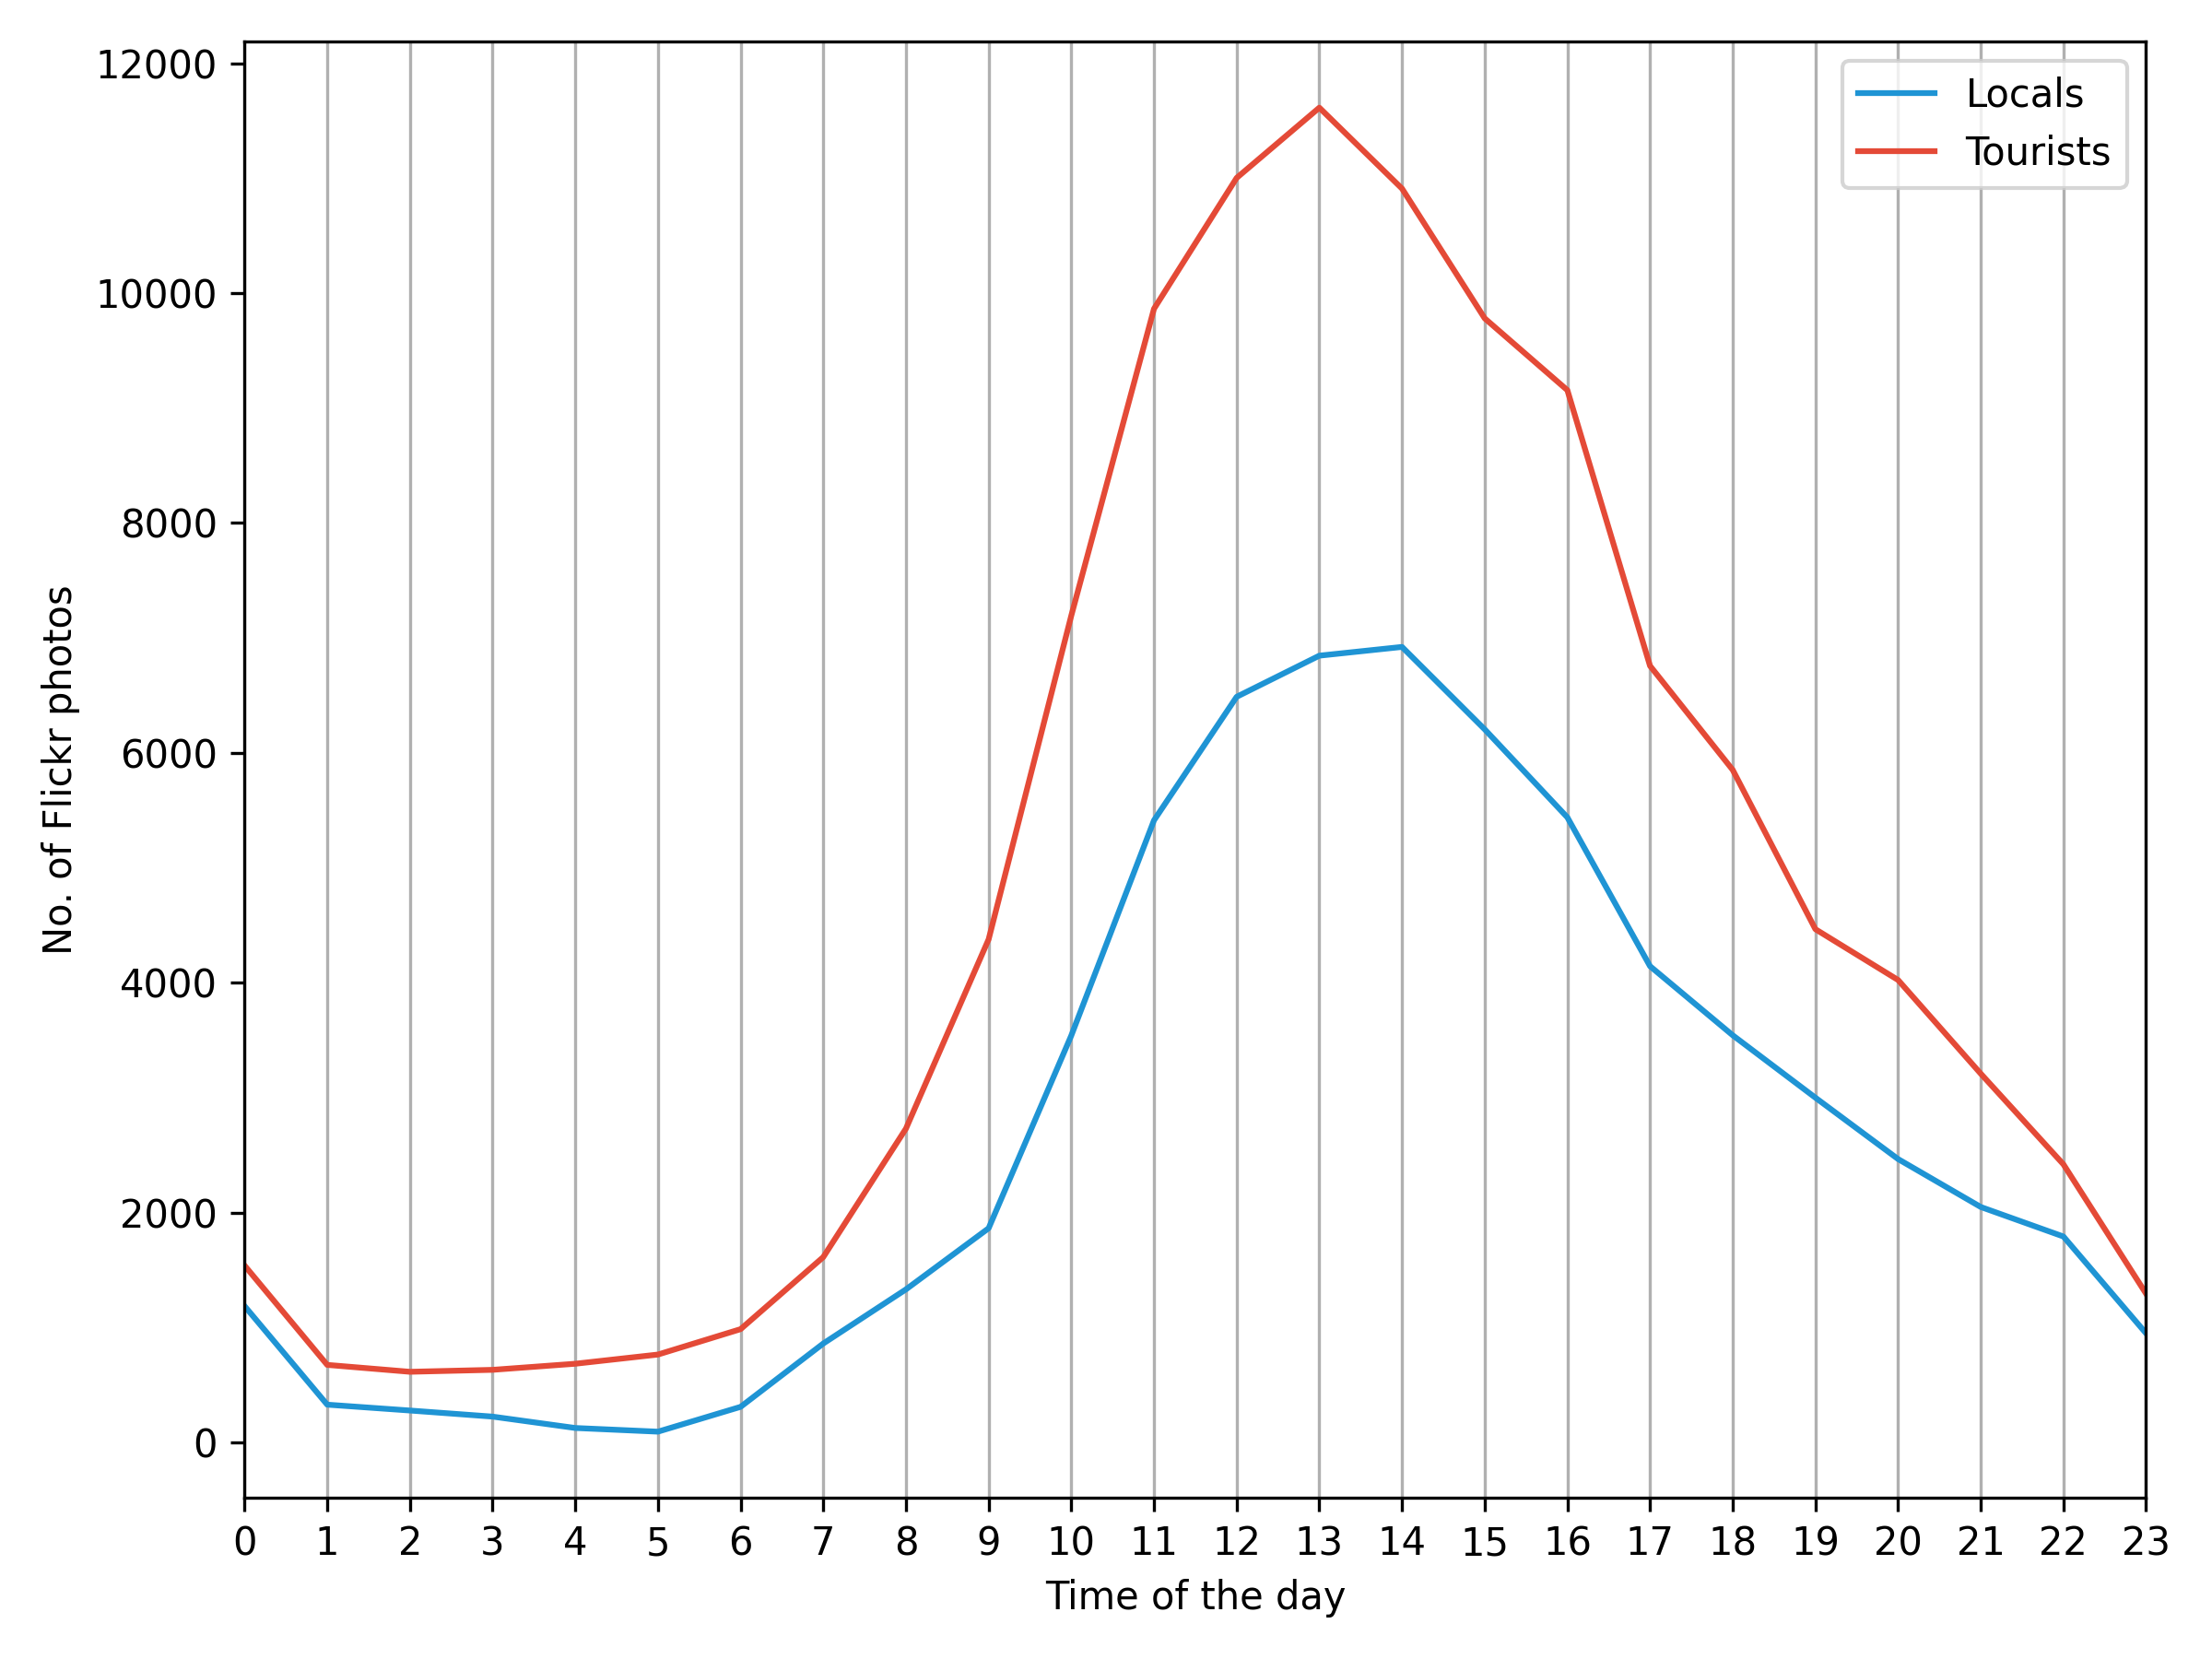
\includegraphics[width=0.8\textwidth]{figures/flickr_trend_day.png}
\caption{\label{fig:flickr_trend_day}Temporal Flickr photos sharing pattern along the day.}
\end{figure}

Figure \ref{fig:flickr_trend_week}
\begin{figure}
\centering
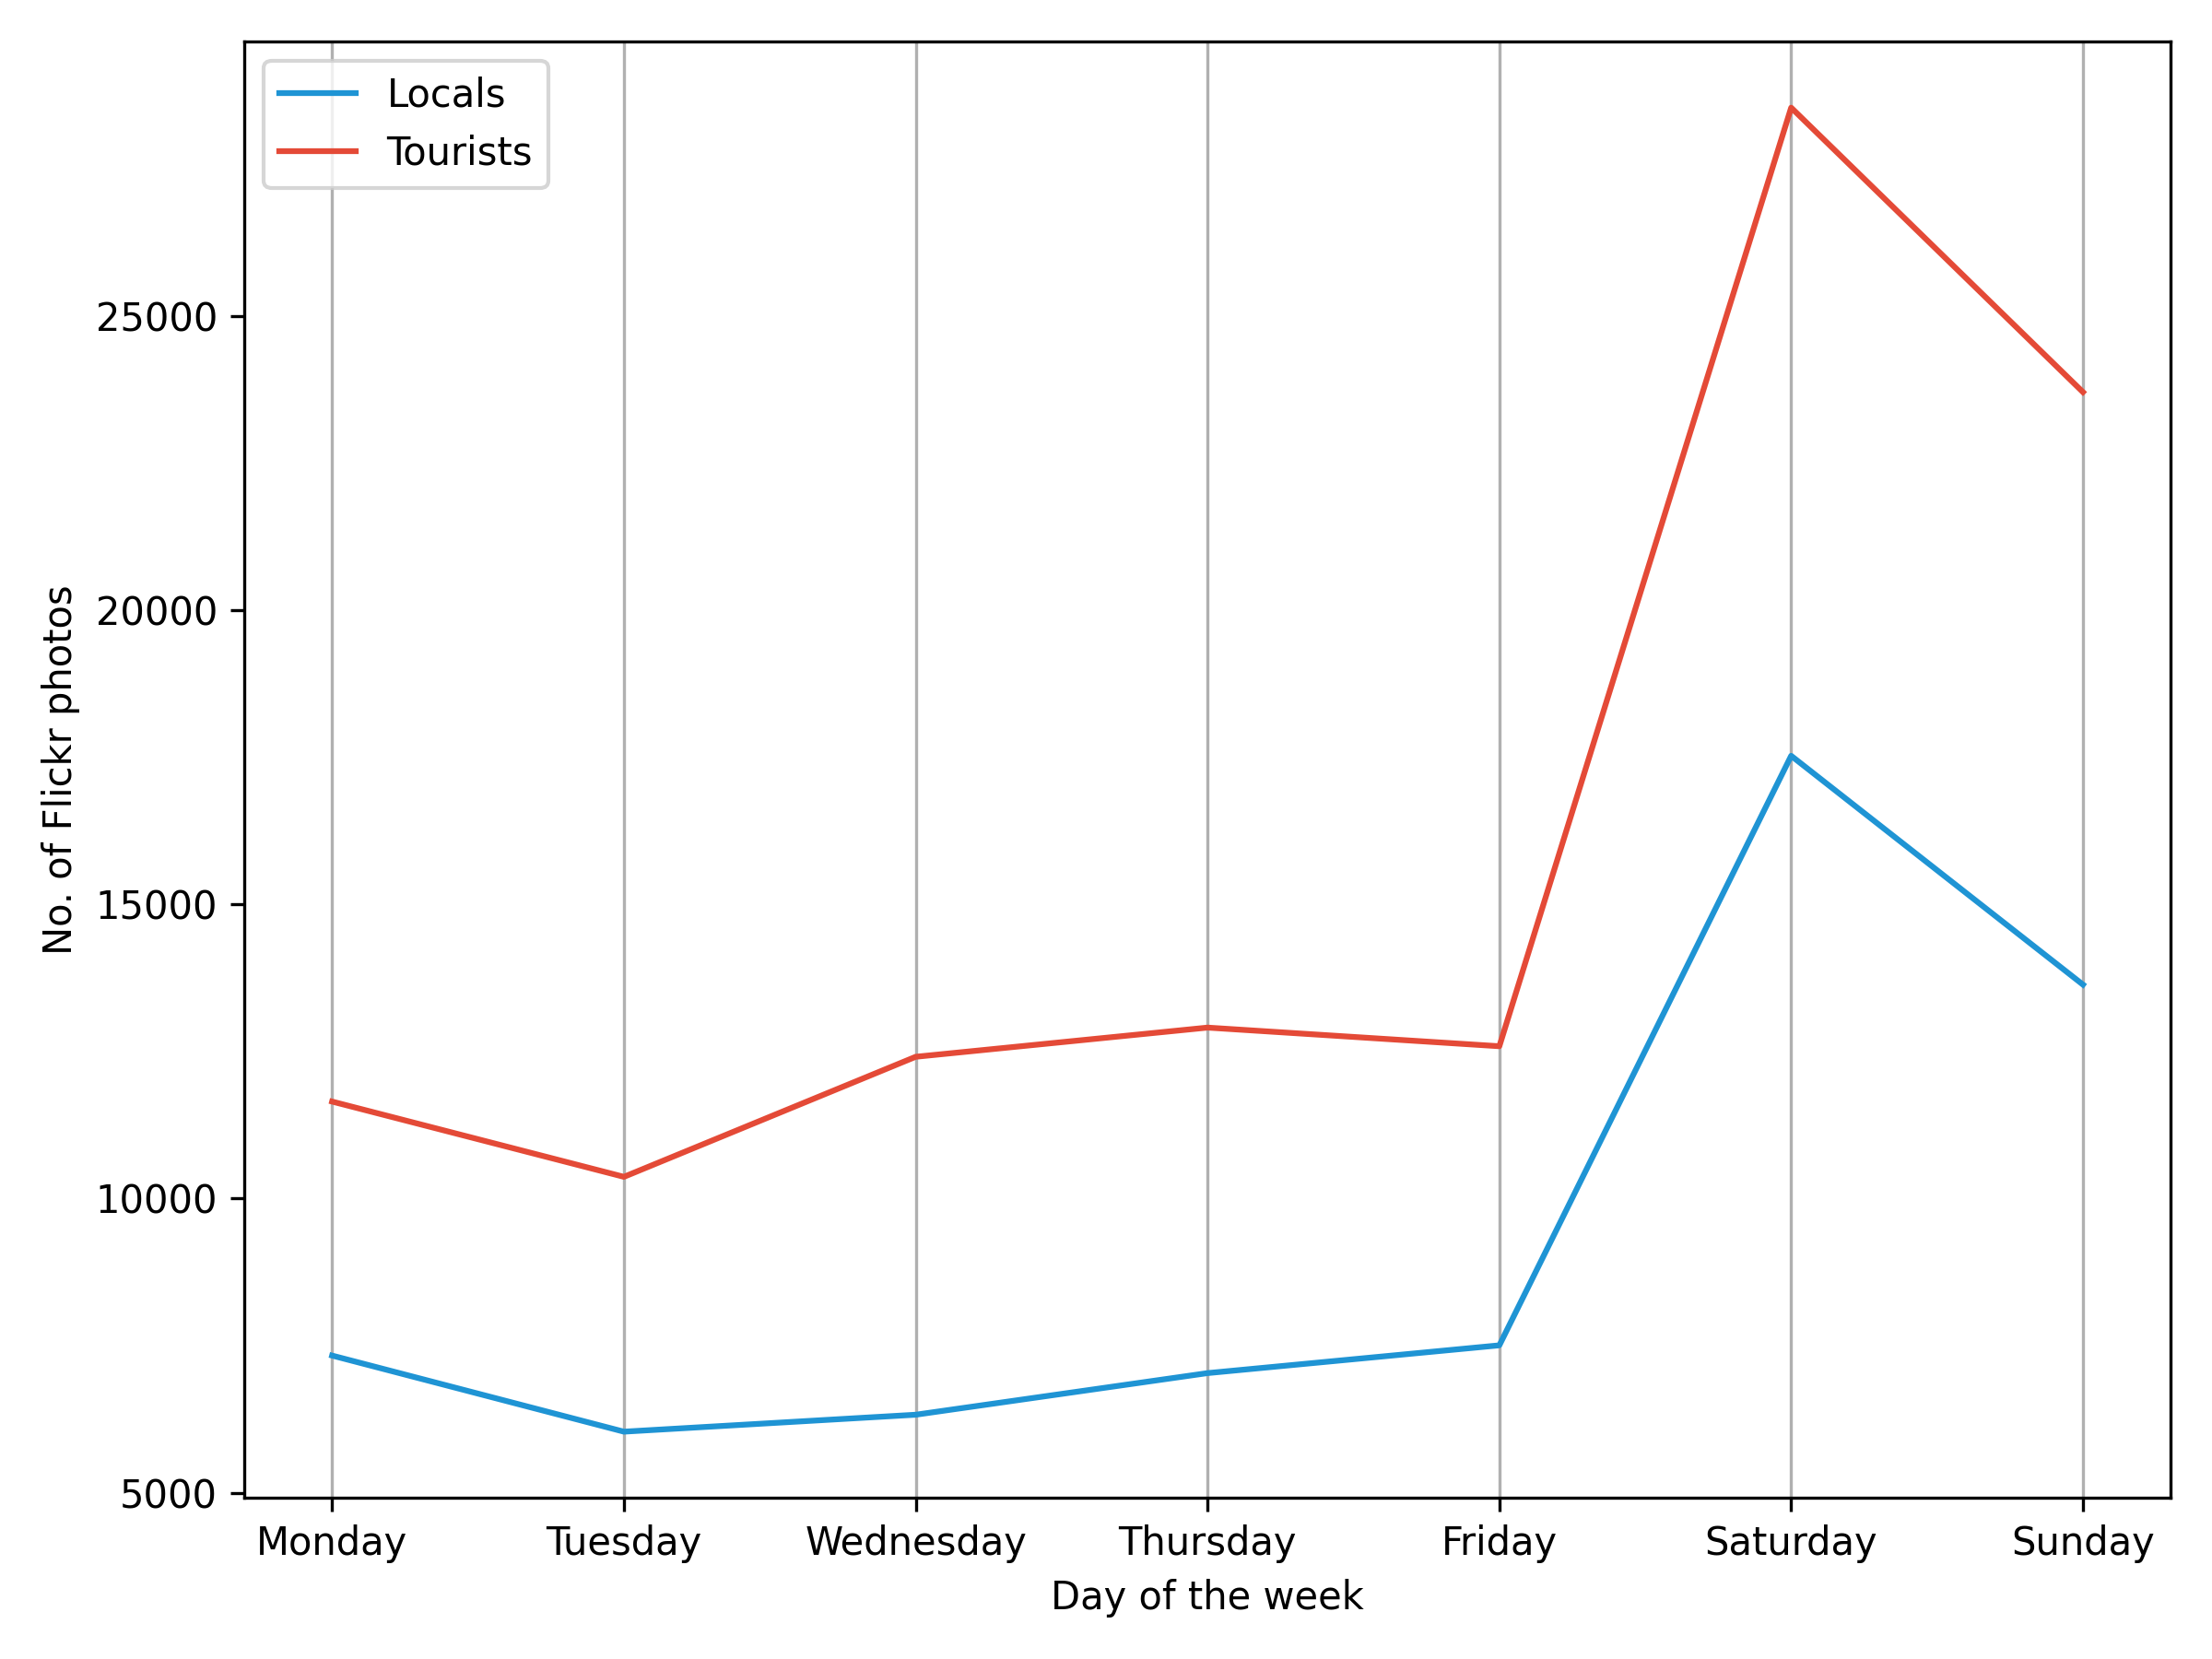
\includegraphics[width=0.8\textwidth]{figures/flickr_trend_week.png}
\caption{\label{fig:flickr_trend_week}Temporal Flickr photos sharing pattern along the week.}
\end{figure}
\newpage


\section{Discussion}
\subsection{Research Question 1}

\subsection{Research Question 2}

\subsection{Limitations}
limitation: foursquare is not for everyone, most users are young people


\newpage


\section{Conclusion}
\newpage



\pagenumbering{roman}

\bibliographystyle{apacite}
\bibliography{references}

\newpage
\section{Appendix}

\end{document}